% =====================================================================
%  AI Kaizen Copilot — Motion Analyzer · Báo cáo môn Học máy nâng cao (1 cột)
%  Biên dịch:  cd docs/report && latexmk        (XeLaTeX, xem latexmkrc) → build/main.pdf
%  Ảnh: figures/*.png · Sơ đồ TikZ: figures/*.tex · Tài liệu tham khảo: references.bib
%  Ô cần bổ sung đánh dấu \todo{...} (chữ đỏ) và \tbd (dấu ? đỏ trong bảng).
% =====================================================================
\documentclass[12pt,a4paper]{article}

% ---------- Thông tin bìa (sửa ở đây) ----------
\newcommand{\truong}{TRƯỜNG ĐẠI HỌC PHENIKAA}
\newcommand{\khoa}{}                               % vd: KHOA CÔNG NGHỆ THÔNG TIN — để trống thì không in
\newcommand{\monhoc}{HỌC MÁY NÂNG CAO}
\newcommand{\mamonhoc}{\todo{bổ sung}}
\newcommand{\giangvien}{PGS.TS Phạm Tiến Lâm}
\newcommand{\detai}{AI Kaizen Copilot: Định lượng Muda--Mura--Muri\\ từ video lắp ráp với giải thích LLM có kiểm chứng}
\newcommand{\noithoigian}{Hà Nội, tháng 11 năm 2026}

% ---------- Trang + font + tiếng Việt (XeLaTeX) ----------
\usepackage[a4paper,left=3cm,right=2cm,top=2.5cm,bottom=2.5cm]{geometry}
\usepackage{fontspec}
\usepackage[vietnamese,english]{babel}
\setmainfont{TeX Gyre Termes}
\setsansfont{TeX Gyre Heros}
\setmonofont{TeX Gyre Cursor}[Scale=0.95]
\babelprovide[main,import]{vietnamese}
\AtBeginDocument{\renewcommand{\figurename}{Hình}\renewcommand{\tablename}{Bảng}%
  \renewcommand{\abstractname}{Abstract}\renewcommand{\refname}{References}%
  \renewcommand{\contentsname}{Mục lục}}
\usepackage{setspace}
\setstretch{1.25}
\setlength{\parskip}{3pt}
\setlength{\emergencystretch}{3em}               % tránh tràn lề khi có tên file / mã dài

% ---------- Gói chung ----------
\usepackage{amsmath,amssymb}
\usepackage{graphicx}
\graphicspath{{figures/}}
\usepackage{booktabs,multirow,tabularx,array}
\usepackage{adjustbox}
\usepackage[table]{xcolor}
\usepackage{tikz}
\usetikzlibrary{positioning,arrows.meta,fit,backgrounds,calc,shapes.geometric}
\usepackage{algorithm}
\usepackage{algpseudocode}
\usepackage[font=small,labelfont=bf]{caption}
\usepackage{float}
\usepackage{fancyvrb}
\usepackage{url}
\usepackage{xurl}                                  % ngắt dòng URL dài trong References
\usepackage[hidelinks]{hyperref}
\urlstyle{same}
\usepackage{cleveref}

% ---------- Macro ----------
\newcommand{\todo}[1]{\textcolor{red}{\textbf{[TODO:} #1\textbf{]}}}
\newcommand{\tbd}{\textcolor{red}{\textbf{?}}}   % ô bảng chờ điền số
\newcommand{\code}[1]{\texttt{#1}}
\newcommand{\muda}{\textit{Muda}}
\newcommand{\mura}{\textit{Mura}}
\newcommand{\muri}{\textit{Muri}}
\newcommand{\Fone}{F1@IoU0.5}
\newenvironment{IEEEkeywords}{\par\smallskip\noindent\textbf{Từ khoá:}~}{\par}
\renewcommand{\algorithmicrequire}{\textbf{Vào:}}
\renewcommand{\algorithmicensure}{\textbf{Ra:}}
\crefname{figure}{Hình}{Hình}
\crefname{table}{Bảng}{Bảng}
\crefname{section}{Mục}{Mục}
\crefname{subsection}{Mục}{Mục}
\crefname{equation}{}{}
\crefname{algorithm}{Thuật toán}{Thuật toán}

\begin{document}

% ============================== BÌA ==============================
\begin{titlepage}
  \centering
  {\large\bfseries \truong\par}
  \ifx\khoa\empty\else{\large\bfseries \khoa\par}\fi
  \vspace{0.3cm}\rule{0.6\textwidth}{0.6pt}\par
  \vspace{1.2cm}
  \IfFileExists{figures/logo.png}{\includegraphics[height=3.5cm]{logo.png}\par\vspace{1cm}}{\vspace{2cm}}
  {\Large\bfseries BÁO CÁO MÔN HỌC\par}
  \vspace{0.4cm}
  {\LARGE\bfseries \monhoc\par}
  \vspace{0.3cm}
  {\large Mã môn học: \mamonhoc\par}
  \vspace{1.5cm}
  {\large\bfseries ĐỀ TÀI\par}
  \vspace{0.3cm}
  {\Large\bfseries \detai\par}
  \vfill
  \begin{tabular}{@{}ll@{}}
    \textbf{Giảng viên hướng dẫn:} & \giangvien \\[0.4cm]
    \textbf{Sinh viên thực hiện:}  & \begin{tabular}[t]{@{}ll@{}}
                                       Trịnh Gia Huy (Nhóm trưởng) & MSSV: \todo{} \\
                                       Nguyễn Thị Nhung            & MSSV: \todo{} \\
                                       Hoàng Tiến Đạt              & MSSV: \todo{} \\
                                     \end{tabular}
  \end{tabular}
  \vfill
  {\large \noithoigian\par}
\end{titlepage}

% ============================== TÓM TẮT + MỤC LỤC ==============================
\pagenumbering{roman}
\setcounter{page}{2}
\addcontentsline{toc}{section}{Abstract}
% ============================== ABSTRACT ==============================
 
\begin{abstract}
Trong sản xuất, đo thời gian thao tác thủ công thường mất 2--4 giờ mỗi trạm và chỉ ghi nhận được một số chu kỳ, khiến việc theo dõi liên tục lãng phí (\muda), biến động (\mura) và quá tải (\muri) gặp nhiều hạn chế.

Chúng tôi đề xuất \textit{AI Kaizen Copilot}, hệ thống chuyển video RGB tại trạm lắp ráp thành các chỉ số Kaizen và đề xuất cải tiến có trích dẫn nguồn. Pipeline gồm ba tầng: (i) \textit{Skeleton} sử dụng MediaPipe, RTMW hoặc RTMPose để ước lượng và xử lý quỹ đạo khung xương 2D, từ đó nhận diện các sự kiện thao tác; (ii) \textit{Analyzer} phân đoạn chu kỳ thành 12 bước SOP bằng luật hoặc MS-TCN, tính toán cycle time, \%VA, quãng đường tay và độ biến thiên, đồng thời áp dụng tám quy tắc (R1--R8) để phát hiện và xếp hạng vấn đề; (iii) \textit{LLM} kết hợp RAG để diễn giải kết quả và trích dẫn hướng dẫn công việc. Đầu ra được kiểm chứng bằng code nhằm đảm bảo tính nhất quán của số liệu và nguồn tham chiếu.

Thử nghiệm trên HA4M (lắp ráp bộ bánh răng hành tinh, Azure Kinect, 30 fps) cho thấy baseline luật đạt F1 lần lượt 0,75 và 0,714 trong nhận diện sự kiện và phân đoạn bước SOP; MAE thời lượng bước đạt 0,62--0,92 s, sai số cycle time đạt 0,6--2,27 s. Gemini 2.5 Flash đạt tỷ lệ kiểm chứng 100\% sau tối đa một lần hỏi lại. Hệ thống phát hiện bước 9 và 12 chậm hơn chuẩn lần lượt 76,1\% và 34,3\% trong chu kỳ lắp ráp thứ hai. Kết quả MS-TCN sẽ được trình bày tại \cref{sec:exp}.
\end{abstract}

\begin{IEEEkeywords}
Kaizen, Muda--Mura--Muri, ước lượng khung xương, phân đoạn hành động theo thời gian, MS-TCN, HA4M,
mô hình ngôn ngữ lớn, truy xuất tăng cường (RAG), kiểm chứng đầu ra LLM.
\end{IEEEkeywords}

\clearpage
\tableofcontents
\clearpage
\pagenumbering{arabic}

% ============================== NỘI DUNG ==============================
% Sinh từ cùng nguồn nội dung với bản Word.
\section{Introduction}

\subsection{Background and Motivation}

Trong lắp ráp, tổng thời gian hoàn thành một chu kỳ phản ánh năng suất chung nhưng không cho biết thời gian được phân bổ thế nào giữa các bước như lấy linh kiện, định vị, lắp ghép hay dùng dụng cụ. Muốn biết vì sao một chu kỳ kéo dài, cần nhận ra từng thao tác, mốc bắt đầu, kết thúc của nó và các khoảng chờ hay thao tác lặp.

Hiện nay việc này thường làm bằng cách quan sát hoặc xem lại video, bấm giờ và ghi chép. Cách làm tốn thời gian khi số video tăng, và mỗi người đánh giá có thể chọn mốc bắt đầu, kết thúc khác nhau nên số liệu kém nhất quán. Một công cụ tự động nhận dạng và đo thời gian từng bước giúp giảm việc thủ công và tạo cơ sở so sánh thống nhất.

Ước lượng tư thế người cho phép biểu diễn chuyển động bằng chuỗi điểm khớp, từ đó mô hình học có thể nhận dạng thao tác và ranh giới thời gian của chúng. Tuy nhiên, nhận dạng thao tác lắp ráp có những khó khăn riêng: nhiều bước có động tác gần giống nhau nhưng khác linh kiện, một số thao tác lặp lại liên tiếp trong cùng chu kỳ, và bàn tay thường bị che khuất. Sau khi đo được thời gian, kết quả còn cần được đặt trong ngữ cảnh của quy trình chuẩn — vốn nằm trong tài liệu hướng dẫn công việc và SOP — để người phụ trách biết bước nào lệch chuẩn và nên cải tiến theo hướng nào. Dự án vì vậy kết hợp phân đoạn hành động từ chuỗi khung xương với truy xuất tăng cường sinh (RAG) để tạo báo cáo có căn cứ và truy vết được, phục vụ hoạt động Kaizen.

\subsection{Problem Statement}

Đầu vào của hệ thống là video RGB ghi một chu kỳ lắp ráp bộ bánh răng hành tinh tại một trạm cố định, định nghĩa 12 bước thao tác và tập tài liệu tham chiếu. Nhiệm vụ thứ nhất là học có giám sát: dự đoán nhãn bước và lần lặp tại từng khung hình từ chuỗi điểm khớp, rồi chuyển thành các đoạn có mốc bắt đầu, kết thúc. Nhiệm vụ thứ hai là đánh giá: tính thời lượng từng bước, đối chiếu với thời gian chuẩn truy xuất từ tài liệu, phát hiện các bước lệch ngưỡng và sinh khuyến nghị cải tiến có trích dẫn. Mọi phép tính thời gian và chênh lệch do chương trình thực hiện; mô hình ngôn ngữ chỉ diễn giải các số liệu đã tính và đoạn tài liệu đã truy xuất.

Câu hỏi nghiên cứu trọng tâm là: (i) mô hình phân đoạn học từ khung xương 2D có khái quát sang người thực hiện chưa xuất hiện khi huấn luyện hay không, và những yếu tố nào của dữ liệu giới hạn khả năng đó; (ii) sai số phân đoạn ảnh hưởng thế nào đến các phát hiện và khuyến nghị mà tầng RAG tạo ra.

\subsection{Objectives and Scope}

Mục tiêu là xây dựng và đánh giá thực nghiệm một luồng xử lý thống nhất từ video đến báo cáo khuyến nghị, gồm: trích xuất điểm khớp, phân đoạn bước bằng MS-TCN, đo thời lượng, truy xuất tài liệu chuẩn và sinh diễn giải có kiểm tra. Dự án được phát triển cho cuộc thi DENSO Factory Hacks 2026~\citep{denso}. Phạm vi dữ liệu là nhiệm vụ lắp ráp bộ bánh răng hành tinh của bộ dữ liệu HA4M~\citep{ha4m} với một góc camera cố định; tại thời điểm thực nghiệm, nhóm có ba video có nhãn của hai người (hai video của U001 và một video của U002), nên kết quả được trình bày như một nghiên cứu thí điểm, với người huấn luyện và người kiểm tra tách riêng. Thời gian chuẩn lấy từ tài liệu hướng dẫn công việc do nhóm biên soạn mô phỏng, dùng để kiểm chứng chức năng đối chiếu chứ không đại diện cho định mức của nhà máy.

\subsection{Contributions}

Đóng góp của đề tài mang tính thực nghiệm: (1) một luồng xử lý hoàn chỉnh, có lưu vết từ khung hình đến khuyến nghị; (2) một giao thức đánh giá tách người khi số người rất ít — kiểm định chéo theo video trên người huấn luyện để chọn siêu tham số, kiểm tra trên người mới, 5 seed cho mỗi cấu hình — cùng so sánh với kết quả kiểm tra trong cùng người; (3) phân tích nguyên nhân suy giảm khái quát (găng tay làm hỏng điểm bàn tay, khác biệt tốc độ thao tác) và các biện pháp tương ứng — loại nhóm đặc trưng kém tin cậy, tăng cường co giãn tốc độ, giải mã ràng buộc thứ tự SOP — được đo bằng nghiên cứu loại bỏ thành phần; (4) thiết kế và phân tích định tính tầng RAG, gồm cơ chế kiểm tra đầu ra và đối chiếu phát hiện giữa ranh giới dự đoán và ranh giới chuẩn.

% Sinh từ cùng nguồn nội dung với bản Word.
\section{Overview and Related Work}

\subsection{Pose Estimation for Assembly Video}

Ước lượng tư thế người xác định toạ độ các điểm khớp trong ảnh. BlazePose~\citep{blazepose} là mô hình nhẹ dự đoán 33 điểm cơ thể, kết hợp giám sát bằng bản đồ nhiệt khi huấn luyện với hồi quy toạ độ khi suy luận; đây là mô hình nền của bộ Pose Landmarker trong MediaPipe được dùng trong hệ thống. MediaPipe Hands~\citep{mphands} phát hiện lòng bàn tay rồi hồi quy 21 điểm trên mỗi bàn tay. Cả hai được huấn luyện trên ảnh người với bàn tay trần và tư thế thông thường, nên chất lượng điểm khớp trong môi trường lắp ráp — bàn tay nhỏ trong ảnh, bị linh kiện che, hoặc đeo găng — cần được đo trực tiếp thay vì giả định. Ở Chương V, chất lượng điểm bàn tay là một trong những nguyên nhân chính làm mô hình phía sau kém khi chuyển sang người mới.

\subsection{Temporal Action Segmentation}

Phân đoạn hành động theo thời gian gán nhãn cho mọi khung hình của một video dài chứa nhiều hành động nối tiếp. MS-TCN~\citep{farha2019mstcn} xếp chồng nhiều giai đoạn tích chập một chiều có hệ số giãn tăng gấp đôi; giai đoạn đầu nhận đặc trưng khung hình, các giai đoạn sau tinh chỉnh phân bố xác suất của giai đoạn trước. Hàm mất mát kết hợp cross-entropy với thành phần làm mượt T-MSE nhằm giảm hiện tượng phân mảnh. Kiến trúc này phù hợp với bài toán vì vùng tiếp nhận đủ bao trùm cả chu kỳ lắp ráp, số tham số nhỏ (dưới 0,7 triệu) và có thể huấn luyện với rất ít video. Các hướng khác như mạng tích chập đồ thị trên khung xương hay kiến trúc Transformer cho phân đoạn thường có nhiều tham số hơn; với ba video có nhãn, nhóm không thử các hướng này.

\subsection{Retrieval-Augmented Generation and Vector Stores}

RAG bổ sung tri thức ngoài cho mô hình ngôn ngữ bằng cách truy xuất các đoạn tài liệu liên quan và đưa vào ngữ cảnh sinh. Chất lượng truy xuất phụ thuộc vào bộ mã hoá văn bản: multilingual-E5~\citep{e5} là họ mô hình mã hoá đa ngôn ngữ huấn luyện tương phản, phân biệt truy vấn và đoạn văn bằng tiền tố, phù hợp với tài liệu tiếng Việt. Các vector được lưu và tìm kiếm lân cận gần đúng trong ChromaDB~\citep{chroma}, một cơ sở dữ liệu vector nhúng chạy cục bộ, lưu kèm metadata để truy vết nguồn. Ở thành phần sinh, hệ thống dùng mô hình Gemini~\citep{gemini2023,geminidocs} qua API, không tinh chỉnh. Khác với các ứng dụng hỏi đáp, ở đây đầu vào của RAG là các phát hiện định lượng do chương trình tính, nên yêu cầu then chốt là mô hình ngôn ngữ không được tạo số liệu mới và mọi nhận định phải dẫn được về đoạn tài liệu.

% ============================== III. METHOD ==============================
\section{Method}
\label{sec:method}

\begin{figure}[t]
  \centering
  \resizebox{\textwidth}{!}{% Sơ đồ kiến trúc tổng thể (TikZ) — dùng trong figure* ở sections/03_method.tex
\begin{tikzpicture}[
  font=\scriptsize,
  >={Stealth[length=2mm]},
  box/.style={draw, rounded corners=2pt, align=center, minimum width=2.9cm, minimum height=0.95cm,
              inner sep=2pt, fill=white},
  nin/.style={box, fill=gray!10},
  nout/.style={box, fill=green!8},
  llm/.style={box, fill=orange!10},
  grp/.style={draw=#1!60, fill=#1!5, rounded corners=4pt, inner sep=6pt},
  lab/.style={font=\scriptsize\bfseries, text=#1!70!black},
  flow/.style={->, thick},
  aux/.style={->, densely dashed, gray!70!black},
]
% ---- cột 0: đầu vào
\node[nin] (lab)  at (0, 1.35)  {\textbf{Labels.txt} (HA4M)\\nhãn theo frame};
\node[nin] (vid)  at (0, 0)     {\textbf{Video RGB}\\.mp4 $|$ chuỗi ảnh $|$ HA4M};
\node[nin] (st)   at (0, -1.3)  {\textbf{station.yaml}\\zone, 12 bước SOP, VA};
\node[nin] (doc)  at (0, -3.9)  {\textbf{Tài liệu}\\WI / SOP / KB (PDF, DOCX, MD)};

% ---- cột 1: tầng skeleton
\node[box] (s1) at (3.75, 0)    {\textbf{01 Pose}\\MediaPipe $|$ RTMW $|$ RTMPose-ft};
\node[box] (s2) at (3.75, -1.3) {\textbf{02 Features}\\lọc, One Euro, tốc độ, zone};
\node[box] (s3) at (3.75, -2.6) {\textbf{03 Events}\\pick / reach / assemble / idle};

% ---- cột 2: tầng analyzer
\node[box] (a1) at (7.5, 0)     {\textbf{04 Steps}\\oracle $|$ rule $|$ MS-TCN};
\node[box] (a2) at (7.5, -1.3)  {\textbf{05 Metrics}\\Muda $\cdot$ Mura $\cdot$ Muri};
\node[box] (a3) at (7.5, -2.6)  {\textbf{06 Findings}\\R1--R8, xếp hạng s/chu kỳ};

% ---- cột 3: tầng LLM
\node[llm] (l2) at (11.25, -1.3) {\textbf{Validator}\\whitelist số + citation};
\node[llm] (l1) at (11.25, -2.6) {\textbf{07 Explain}\\Gemini $|$ Claude $|$ GPT};
\node[llm] (l0) at (11.25, -3.9) {\textbf{RAG store}\\chunk $\to$ e5 $\to$ Chroma};

% ---- cột 4: đầu ra
\node[nout] (o0) at (15.0, 0)    {\textbf{Run}\\manifest + artifact};
\node[nout] (o1) at (15.0, -1.3) {\textbf{08 Report}\\Markdown + PNG};
\node[nout] (o2) at (15.0, -2.6) {\textbf{UI / API}\\Streamlit, FastAPI};

% ---- nhóm tầng
\begin{scope}[on background layer]
  \node[grp=blue,   fit=(s1)(s3), label={[lab=blue]above:Tầng 1 — skeleton}] {};
  \node[grp=violet, fit=(a1)(a3), label={[lab=violet]above:Tầng 2 — analyzer (tất định)}] {};
  \node[grp=orange, fit=(l2)(l0), label={[lab=orange]above:Tầng 3 — LLM}] {};
\end{scope}

% ---- luồng chính
\draw[flow] (vid) -- node[above]{\tiny frame} (s1);
\draw[flow] (s1) -- node[right]{\tiny .npz} (s2);
\draw[flow] (s2) -- node[right]{\tiny .parquet} (s3);
\draw[flow] (s3.east) -- ++(0.35,0) |- (a1.west);
\draw[flow] (a1) -- node[right]{\tiny steps.csv} (a2);
\draw[flow] (a2) -- node[right]{\tiny metrics.json} (a3);
\draw[flow] (a3) -- node[above]{\tiny findings} (l1);
\draw[flow] (l1.north) -- (l2.south);
\draw[->, thick, red!70!black] (l2.east) .. controls +(0.55,-0.3) and +(0.55,0.3) .. node[right, align=left]{\tiny fail $\to$\\[-2pt]\tiny hỏi lại 1 lần} (l1.east);
\draw[flow] (l2) -- node[above]{\tiny passed} (o1);
\draw[flow] (o1) -- (o2);
\draw[aux]  (o1) -- (o0);
\draw[flow] (l0) -- node[right]{\tiny top-$k$ chunk} (l1);

% ---- luồng phụ
\draw[aux] (lab.east) -- (a1.north |- lab.east) node[pos=0.5, above]{\tiny chế độ oracle / eval} -- (a1.north);
\draw[aux] (st) -- node[above]{\tiny zone} (s2);
\draw[aux] (doc) -- node[above]{\tiny ingest (heading-aware 300--600 token)} (l0);
\draw[aux] ($(l0.west)+(0,0.22)$) -| node[pos=0.8, right]{\tiny TG chuẩn + ngưỡng} ($(a3.south)+(0.8,0)$);
\end{tikzpicture}
}
  \caption{Kiến trúc tổng thể AI Kaizen Copilot. Mỗi khối 01--08 là một chương trình đọc file vào và ghi file ra
  trong cùng một \textit{run} có manifest.
  Tầng 2 hoàn toàn tất định (không gọi LLM hay mạng). LLM ở tầng 3 chỉ diễn giải, và mọi câu trả lời phải qua validator.
  \code{station.yaml} còn cung cấp danh sách bước SOP và cờ VA cho khối 04--06.
  Đường nét đứt là dữ liệu phụ: nhãn HA4M cho chế độ oracle và đánh giá, thời gian chuẩn lấy từ tài liệu qua RAG.}
  \label{fig:arch}
\end{figure}

\subsection{Phát biểu bài toán}
\label{subsec:problem}
Đầu vào gồm ba phần:
\begin{itemize}
  \item video RGB $V=\{I_t\}_{t=1}^{T}$ của một trạm có một công nhân, tốc độ $f$ frame/s;
  \item cấu hình trạm $\mathcal{S}$, gồm tập vùng (zone) đa giác $\{Z_k\}$ trên ảnh (khay linh kiện, vùng lắp)
        và chuỗi bước SOP $\langle (j, \text{tên}_j, Z_{(j)}, \text{va}_j, \text{rep}_j)\rangle_{j=1}^{12}$;
  \item một kho tài liệu $\mathcal{D}$ (work instruction, SOP, cơ sở tri thức Kaizen).
\end{itemize}
Hệ thống cần xuất ra:
(a) phân đoạn chu kỳ thành các bước $\{(j, r, s_{j,r}, e_{j,r})\}$, với $r$ là lần lặp (ví dụ bước 2 lặp 3 lần);
(b) tập chỉ số $\mathcal{M}$, mỗi chỉ số có giá trị, đơn vị và định nghĩa;
(c) tập phát hiện $\mathcal{F}$, mỗi phát hiện kèm bằng chứng, ảnh hưởng (giây/chu kỳ) và độ tin cậy;
(d) với mỗi $f\in\mathcal{F}$, một giải thích $\langle$quan sát, giả thuyết, đề xuất, ECRS, trích dẫn$\rangle$
đã qua kiểm chứng.
Ràng buộc then chốt: mọi số xuất hiện trong (d) phải truy ngược được về (b)--(c).
\Cref{fig:arch} tóm tắt toàn bộ luồng xử lý.

\subsection{Ước lượng khung xương và làm sạch quỹ đạo cổ tay}
\label{subsec:pose}
Mỗi frame được đưa qua một backend pose trong vùng quan tâm (ROI) cố định của trạm.
Các backend là MediaPipe (33 điểm thân cộng $2\times21$ điểm tay, tổng 75), RTMW (133 điểm) hoặc RTMPose fine-tune (COCO-17).
Đầu ra là tensor $K\in\mathbb{R}^{T\times J\times 3}$ gồm $(x,y,\text{score})$.
Với mỗi cổ tay $h\in\{\text{L},\text{R}\}$, quỹ đạo $p^h_t$ được làm sạch theo bốn bước:
\begin{enumerate}
  \item điểm có score $<0{,}3$ coi là thiếu (NaN);
  \item \textit{điểm gai}, tức điểm mà vận tốc nhảy vào và nhảy ra đều vượt $v_{\max}=2500$\,px/s, bị loại;
  \item đoạn thiếu dài $\le 15$ frame (0{,}5\,s) được nội suy tuyến tính và đánh cờ \code{interp};
        đoạn dài hơn giữ NaN và không tính vào quãng đường;
  \item lọc One Euro \cite{casiez2012oneeuro} trên từng đoạn liên tục.
\end{enumerate}
Bộ lọc One Euro thích nghi tần số cắt theo tốc độ:
\begin{gather}
  \hat{p}_t = \alpha_t p_t + (1-\alpha_t)\hat{p}_{t-1},\qquad
  \alpha_t = \Big(1+\frac{f}{2\pi f_c(t)}\Big)^{-1},\nonumber\\
  f_c(t) = f_{c,\min} + \beta\,\lvert\dot{\hat p}_t\rvert,
  \label{eq:oneeuro}
\end{gather}
với $f_{c,\min}=1$\,Hz và $\beta=0{,}01$.
Tốc độ được tính \textit{sau} khi lọc: $v^h_t = f\,\lVert \hat{p}^h_t-\hat{p}^h_{t-1}\rVert_2$ (px/s).
Vùng của cổ tay là $z^h_t = \arg\{Z_k : \hat{p}^h_t\in Z_k\}$, theo thứ tự ưu tiên khi các đa giác chồng nhau;
nếu cổ tay không nằm trong vùng nào thì $z^h_t=$ \code{none}.

\subsection{Phát hiện sự kiện}
\label{subsec:events}
Trạng thái mỗi tay tại frame $t$ là cặp $\sigma^h_t=(z^h_t, m^h_t)$, trong đó $m\in\{\text{moving},\text{still},\text{lost}\}$
được xác định bằng ngưỡng $v^h_t \gtrless 120$\,px/s; \text{lost} ứng với cổ tay NaN.
Các frame liên tiếp cùng trạng thái được nén (run-length) thành sự kiện.
Sự kiện ngắn hơn $0{,}25$\,s được nhập vào sự kiện kề dài hơn, lặp lại cho tới khi không còn sự kiện ngắn,
rồi gộp các sự kiện kề nhau cùng trạng thái.
Mỗi sự kiện được gán loại theo quy tắc ở \cref{tab:events}.
Các quy tắc này cố ý đơn giản để kỹ sư đọc hiểu và chỉnh được.

\begin{table}[t]
\centering
\caption{Quy tắc suy diễn loại sự kiện (mỗi tay)}
\label{tab:events}
\footnotesize
\begin{tabularx}{\columnwidth}{@{}llX@{}}
\toprule
Vùng & Chuyển động & Loại sự kiện \\
\midrule
khay linh kiện & still $\le 2$\,s & \textit{pick} (lấy) \\
khay linh kiện & still $> 2$\,s  & \textit{search} (tìm) \\
khay linh kiện & moving           & \textit{reach} (với tay) \\
vùng lắp       & bất kỳ           & \textit{assemble} (lắp) \\
vùng thành phẩm & bất kỳ          & \textit{place} (đặt) \\
\code{none}    & still $> 1{,}5$\,s & \textit{idle} (chờ) \\
\code{none}    & still $\le 1{,}5$\,s & \textit{pause} \\
\code{none}    & moving           & \textit{transfer} (di chuyển) \\
--             & lost             & \textit{lost} (mất dấu) \\
\bottomrule
\end{tabularx}
\end{table}

\subsection{Phân đoạn bước SOP}
\label{subsec:steps}
Hệ thống hỗ trợ ba chế độ, đều ghi ra cùng một schema \code{step\_id, repetition, start\_s, end\_s, dur\_s, source}.

\textbf{Oracle.} Đọc nhãn HA4M theo frame. Mỗi đoạn liên tiếp cùng (action, repetition) thành một bước,
với $e = (\text{end\_frame}+1)/f$.

\textbf{Rule (baseline).} Các bước có khay riêng được neo bằng sự kiện lấy linh kiện (\cref{alg:rule}).
Bước không neo được, hoặc có mốc sai thứ tự, được gán \code{unclassified} và ghi vào danh sách bước thiếu.
Chế độ này không cần huấn luyện và giải thích được, nhưng không tách được những bước không có khay đặc trưng
(như bước 9, đặt khối 2 lên khối 1).

\begin{algorithm}[t]
\caption{Phân đoạn bước bằng mốc vùng (rule)}
\label{alg:rule}
\footnotesize
\begin{algorithmic}[1]
\Require Sự kiện $E$ (2 tay), chuỗi SOP $\langle (j,r,Z_{(j)})\rangle$, khoảng cách tối thiểu $\delta$
\Ensure Mốc bắt đầu $a_{j,r}$ cho các bước neo được
\State $t_{\text{prev}}\gets -\infty$
\For{mỗi $(j,r)$ theo thứ tự SOP}
  \If{$Z_{(j)}=\varnothing$} \textbf{đánh dấu} \code{no\_zone}; \textbf{continue} \EndIf
  \State $e^\star \gets$ sự kiện \textit{pick} hoặc \textit{reach} đầu tiên tại $Z_{(j)}$ có $s(e)>t_{\text{prev}}+\delta$
  \If{không có $e^\star$} \textbf{đánh dấu} \code{not\_found}; \textbf{continue} \EndIf
  \State $a_{j,r}\gets$ đầu chuỗi \textit{transfer/reach} liền trước $e^\star$ (lúc tay rời vùng lắp)
  \State $t_{\text{prev}}\gets a_{j,r}$
\EndFor
\State $e_{j,r}\gets$ mốc kế tiếp; bước cuối kết thúc tại sự kiện hoạt động cuối cùng
\State Khoảng giữa các mốc không gán được bước $\to$ \code{unclassified}
\end{algorithmic}
\end{algorithm}

\textbf{MS-TCN (học).} Một mạng MS-TCN \cite{farha2019mstcn} gán nhãn cho từng frame dựa trên đặc trưng khung xương
(\cref{subsec:arch}).
Mỗi lớp là một cặp (action, repetition), cộng thêm lớp nền ``0''.
Sau khi dự đoán, các mảnh bước ngắn hơn $0{,}5$\,s được nhập vào bước kề, trừ mảnh nền.
Sau đó các đoạn được ánh xạ về đúng schema của chế độ rule, nên các khối 05--08 không phải thay đổi.

\textbf{Đánh giá.} Khi có cả dự đoán và oracle, hệ thống ghép từng cặp bước theo $(j,r)$ và tính
$\mathrm{IoU}_{j,r}=\frac{|[s,e]\cap[\hat s,\hat e]|}{|[s,e]\cup[\hat s,\hat e]|}$.
Từ đó suy ra \Fone{} (bước đúng nếu IoU $\ge0{,}5$), MAE thời lượng, MAE mốc bắt đầu và kết thúc,
và sai số cycle time.

\subsection{Chỉ số Kaizen}
\label{subsec:metrics}
Gọi $d_{j}=\sum_r (e_{j,r}-s_{j,r})$ là thời lượng bước $j$.
Mọi chỉ số đều được lưu kèm đơn vị và định nghĩa ngắn; khối 07 đưa nguyên văn các định nghĩa này cho LLM.

\textbf{Muda.}
\begin{align}
  \mathrm{CT} &= e_{\text{cuối}} - s_{\text{đầu}}, \qquad
  \%\mathrm{VA} = 100\cdot\frac{\sum_{j:\,\text{va}_j} d_j}{\mathrm{CT}}, \label{eq:ct}\\
  L^h &= \sum_{t\in\mathcal{T}_{\text{hợp lệ}}} \lVert \hat p^h_t-\hat p^h_{t-1}\rVert_2, \label{eq:path}
\end{align}
trong đó $L^h$ là quãng đường cổ tay (px; đổi sang cm khi có hệ số \code{px\_per\_cm}).
Các chỉ số Muda khác: tổng thời gian idle và transfer của từng tay, số lần lấy theo từng zone trong một chu kỳ.

\textbf{Mura.} Hệ số biến thiên $\mathrm{CV}=\sigma/\mu$ của cycle time và của từng bước, tính giữa các lần lắp
của cùng một người và giữa các người lắp; liệt kê các bước có CV cao nhất.

\textbf{Muri (sàng lọc 2D).} Với khuỷu tay $\mathbf{e}$, cổ tay $\mathbf{w}$ và khớp gốc ngón giữa $\mathbf{m}$
(cùng một tay), góc cổ tay được tính bằng
\begin{equation}
  \theta_t = \arccos\frac{(\mathbf{w}-\mathbf{e})\cdot(\mathbf{m}-\mathbf{w})}
  {\lVert\mathbf{w}-\mathbf{e}\rVert\,\lVert\mathbf{m}-\mathbf{w}\rVert},\qquad
  \Delta_t = \lvert\theta_t - \operatorname{median}(\theta)\rvert .
  \label{eq:muri}
\end{equation}
Hệ thống báo phần trăm thời gian có $\Delta_t>30^\circ$, phân vị 90 của $\Delta$, và độ phủ (tỷ lệ frame đo được).
Đây là góc chiếu 2D, so với trung vị của chính người đó; nó chỉ dùng để sàng lọc, không thay thế
đánh giá công thái học chuyên sâu như RULA.

\subsection{Phát hiện bằng quy tắc}
\label{subsec:findings}
Tám quy tắc ở \cref{tab:rules} chạy trên các chỉ số.
Thêm một quy tắc chỉ cần thêm một phần tử vào danh sách \code{RULES}.
Mỗi phát hiện ghi bằng chứng (chỉ số, giá trị, đơn vị, trial, các mốc thời gian), ảnh hưởng $I$ (giây/chu kỳ)
và độ tin cậy $c\in\{\text{high},\text{med},\text{low}\}$.
Mức nghiêm trọng là \textit{high} nếu $I/\mathrm{CT}\ge5\%$, \textit{med} nếu $I/\mathrm{CT}\ge2\%$, còn lại là \textit{low}.
Danh sách phát hiện được xếp hạng theo
\begin{equation}
  \text{score}(f) = I(f)\cdot w(c),
  \label{eq:rank}
\end{equation}
với $w(\text{high})=1$, $w(\text{med})=0{,}6$, $w(\text{low})=0{,}3$.
Thời gian chuẩn $s^{\text{std}}_j$ và ngưỡng của R8 ưu tiên giá trị ghi trong \code{station.yaml}.
Nếu không có, hệ thống trích từ bảng ``TG chuẩn'' của work instruction trong kho RAG,
và mỗi giá trị đều mang trích dẫn tới trang nguồn.

\begin{table}[t]
\centering
\caption{Các quy tắc phát hiện (V: chạy với 1 video; A: cần nhiều video)}
\label{tab:rules}
\footnotesize
\setlength{\tabcolsep}{3pt}
\begin{tabularx}{\columnwidth}{@{}clXc@{}}
\toprule
ID & Loại & Điều kiện kích hoạt & Phạm vi \\
\midrule
R1 & bước chậm & $d_j > \mathrm{median}+2\cdot\mathrm{MAD}$ (giữa các trial, cần $\ge3$) & A \\
R2 & lấy dư & số pick tại zone $>$ $\sum$ rep của các bước dùng zone đó & V \\
R3 & idle dài & tổng idle 1 tay $>3$\,s/chu kỳ & V \\
R4 & sai thứ tự & chuỗi bước $\neq$ SOP hoặc thiếu bước & V \\
R5 & lệch tay & 1 tay idle $>60\%$ bước khi tay kia hoạt động $>60\%$ & V \\
R6 & biến động & CV cycle time trong 1 người $>0{,}25$ & A \\
R7 & Muri cổ tay & \% thời gian $\Delta_t>30^\circ$ vượt ngưỡng & V \\
R8 & lệch chuẩn & $\lvert d_j-s^{\text{std}}_j\rvert/s^{\text{std}}_j>30\%$ (từ tài liệu) & V \\
\bottomrule
\end{tabularx}
\end{table}

\subsection{Diễn giải bằng LLM có kiểm chứng}
\label{subsec:llm}
\textbf{Prompt.} Prompt có version (\code{explain\_v2}) gồm: định nghĩa chỉ số, phát hiện ở dạng JSON, bảng bước kèm thời gian
chuẩn, và ngữ cảnh tri thức.
Ngữ cảnh tri thức có hai dạng: (a) toàn bộ KB/SOP nhỏ với các đoạn được đánh nhãn \code{[KB-xx]}, \code{[SOP-xx]};
hoặc (b) top-$k$ chunk truy xuất từ kho RAG, mỗi chunk có \code{chunk\_id} dạng \code{DOC-xxxxxx:pN:cM}.
LLM phải trả về JSON thuần gồm quan sát ($\le2$ câu), giả thuyết (1 câu), đề xuất ($\le2$ câu), nhãn ECRS,
hướng dẫn đo lại, và danh sách trích dẫn.

\textbf{Kho tài liệu.} Tài liệu (PDF, DOCX, MD, TXT) được cắt theo heading, mỗi chunk 300--600 token, chồng lấn 50 token.
Mỗi chunk thuộc đúng một trang để trích dẫn chính xác trang; bảng được giữ thành chunk riêng.
Chunk được nhúng bằng multilingual-E5 \cite{e5} và lưu cục bộ trong Chroma \cite{chroma}.

\textbf{Validator.} Với phát hiện $f$, gọi $\mathcal{X}(f)$ là tập các giá trị số trong bằng chứng của nó
và $\mathcal{N}(f)$ là tập số nằm trong tên trường hoặc chuỗi
(ví dụ \code{dev\_p90\_deg}$\to$90, ``lệch $>30^\circ$''$\to$30).
Whitelist của $f$ là
\begin{multline}
  \mathcal{W}(f)=\mathcal{U}\ \cup\ \mathcal{N}(f)\\ \cup \bigcup_{x\in\mathcal{X}(f)}
  \{\mathrm{rd}_0(x), \mathrm{rd}_1(x), \mathrm{rd}_0(|x|), \mathrm{rd}_1(|x|)\},
  \label{eq:whitelist}
\end{multline}
với $\mathcal{U}=\{0,1,2,3,100\}\cup\{1,\dots,12\}$ (số phổ quát và số thứ tự bước), $\mathrm{rd}_k$ là làm tròn
$k$ chữ số thập phân.
Một câu trả lời \textit{đạt} khi cả ba điều kiện sau thoả:
\begin{enumerate}
  \item mọi token số $u$ trong ba trường văn bản thoả $\mathrm{rd}_1(u)\in\mathcal{W}(f)$;
        token dính chữ phía trước như \code{P90}, \code{U001} được bỏ qua;
  \item mọi trích dẫn, sau khi chuẩn hoá (\code{kb13}, \code{[KB-13]} thành \code{KB-13}), tồn tại trong KB/SOP
        hoặc trong kho RAG;
  \item định dạng đúng: số câu nằm trong giới hạn và ECRS $\in\{E,C,R,S\}$.
\end{enumerate}
Nếu không đạt, hệ thống gọi lại LLM \textit{một lần}, kèm thông báo chỉ liệt kê phần sai
(ví dụ ``số lạ: [`8.2']'', ``citation không tồn tại: [`KB-99']'').
Kết quả lưu mọi lần thử cùng trạng thái \code{passed}, \code{failed\_after\_retry} hoặc \code{parse\_failed}.
Pipeline không dừng khi LLM lỗi.
Hai chỉ số được báo cáo là tỷ lệ đạt ngay lần đầu và tỷ lệ đạt sau khi hỏi lại.

\subsection{Báo cáo và truy vết}
Khối 08 sinh báo cáo Markdown gồm: tóm tắt và đề xuất ($\le6$ dòng), bảng bước kèm thời gian chuẩn, độ lệch và nguồn,
biểu đồ Gantt và Yamazumi, 3M tổng hợp, Muri, các phát hiện kèm ảnh bằng chứng, bảng tài liệu tham chiếu
và mục ``Giả định \& giới hạn'' tự sinh.
Ảnh bằng chứng là frame tại thời điểm của phát hiện, có vẽ cổ tay và các zone.
Bảng tài liệu tham chiếu được kiểm tra khớp hai chiều với mọi nhãn trích dẫn trong thân báo cáo.
Mục ``Giả định \& giới hạn'' ghi rõ fps, đơn vị px hay cm, oracle hay dự đoán, và việc Muri chỉ là góc 2D.

% ============================== IV. IMPLEMENTATION ==============================
\section{Implementation}
\label{sec:impl}

\subsection{Code Implementation}
\label{subsec:code}
Hệ thống viết bằng Python~3.11 (khoảng 11 nghìn dòng trong \code{kaizen/}, \code{src/}, \code{app/}).
Thư viện chính: NumPy, pandas, SciPy, Shapely, OneEuroFilter, Matplotlib, OpenCV/MediaPipe, PyTorch (CPU),
Pydantic, ChromaDB, sentence-transformers, FastAPI và Streamlit.
Hệ thống không dùng Docker hay CSDL máy chủ: mọi thứ chạy trên một máy CPU.
Mã nguồn được tổ chức thành một package có ranh giới rõ ràng (\cref{tab:modules}).
Các script \code{src/00\_inspect.py}--\code{src/08\_report.py} chỉ là lớp vỏ CLI mỏng.

\begin{table}[t]
\centering
\caption{Các mô-đun của package \code{kaizen/}}
\label{tab:modules}
\footnotesize
\setlength{\tabcolsep}{3pt}
\begin{tabularx}{\columnwidth}{@{}lX@{}}
\toprule
Mô-đun & Vai trò / API chính \\
\midrule
\code{skeleton} & nguồn video (\code{ha4m://}, \code{video://}, \code{frames://}), backend pose (registry),
                  \code{extract}, \code{compute\_features}, \code{detect\_events}, overlay \\
\code{analyzer} & thuần tính toán: \code{align\_steps}, \code{evaluate}, \code{compute\_metrics},
                  \code{detect\_findings} (\code{RULES} R1--R8), báo cáo, 3M nhiều video \\
\code{llm}      & \code{get\_provider} (anthropic $|$ gemini $|$ openai $|$ dry-run), prompt có version,
                  parse JSON chịu lỗi, \code{validator}, \code{explain} \\
\code{rag}      & ingest PDF/DOCX/MD/TXT $\to$ chunk $\to$ embed $\to$ \code{DocumentStore};
                  trích bước chuẩn, sinh nháp \code{station.yaml} \\
\code{train}    & MS-TCN segmenter, chuẩn bị dữ liệu và đánh giá fine-tune pose \\
\code{core}     & \code{run\_io}, cấu hình, schema Pydantic cho mọi artifact, dự án, pipeline nền \\
\code{api}      & dịch vụ FastAPI (tài liệu, truy vấn RAG, trích bước, diễn giải) \\
\bottomrule
\end{tabularx}
\end{table}

\textbf{Run và truy vết.} Lệnh \code{run\_all.sh} chạy 00$\to$08 vào một thư mục run mới
\code{outputs/runs/<thời điểm>\_<pred|oracle>\_<pose>\_<llm>[\_tag]/} và không ghi đè run cũ.
\code{manifest.json} ghi thời điểm, git hash, lệnh gốc, nguồn dữ liệu, metadata pose, nhãn có sẵn hay không,
provider/model LLM, segmenter và tham số của từng stage.
Bản chụp \code{station.yaml} được lưu cùng run.
Công cụ \code{compare\_runs.py} xuất bảng so sánh cycle time, \%VA, idle, \Fone, MAE và tỷ lệ đạt LLM giữa các run.
Mọi artifact được kiểm bằng schema Pydantic.
Khi refactor, các artifact (\code{metrics.json}, \code{findings.json}, \dots) phải giữ giống từng byte trên cùng một đầu vào.

\textbf{Giao diện.} Ứng dụng Streamlit gồm bốn trang theo mô hình ``một video = một dự án'' (\cref{fig:ui}):
Dự án, Chi tiết dự án (chạy toàn luồng, video overlay, ``Kaizen Brain''), Tài liệu (nạp RAG và thử truy vấn),
và So sánh 3M nhiều video.
UI chỉ đọc artifact qua một lớp truy cập duy nhất và không tự tính bất kỳ chỉ số nào.

\textbf{Kiểm thử.} Bộ \code{pytest} gồm 124 kiểm thử trên dữ liệu tổng hợp (keypoint giả dạng hình sin).
Bộ này bao phủ validator, provider LLM (dùng FakeProvider), các quy tắc R1--R8, adapter pose, RAG, API, UI và
smoke-train MS-TCN, và không cần mạng, API key hay dataset.
Lệnh chạy thử toàn luồng:
\begin{Verbatim}[fontsize=\scriptsize,frame=single]
bash run_all.sh --oracle --subjects U001 --trials all \
     --provider gemini --tag demo
bash run_all.sh --segmenter mstcn \
     --segmenter-model models/segmenter/<name> --dry-run
\end{Verbatim}

\begin{figure}[t]
  \centering
  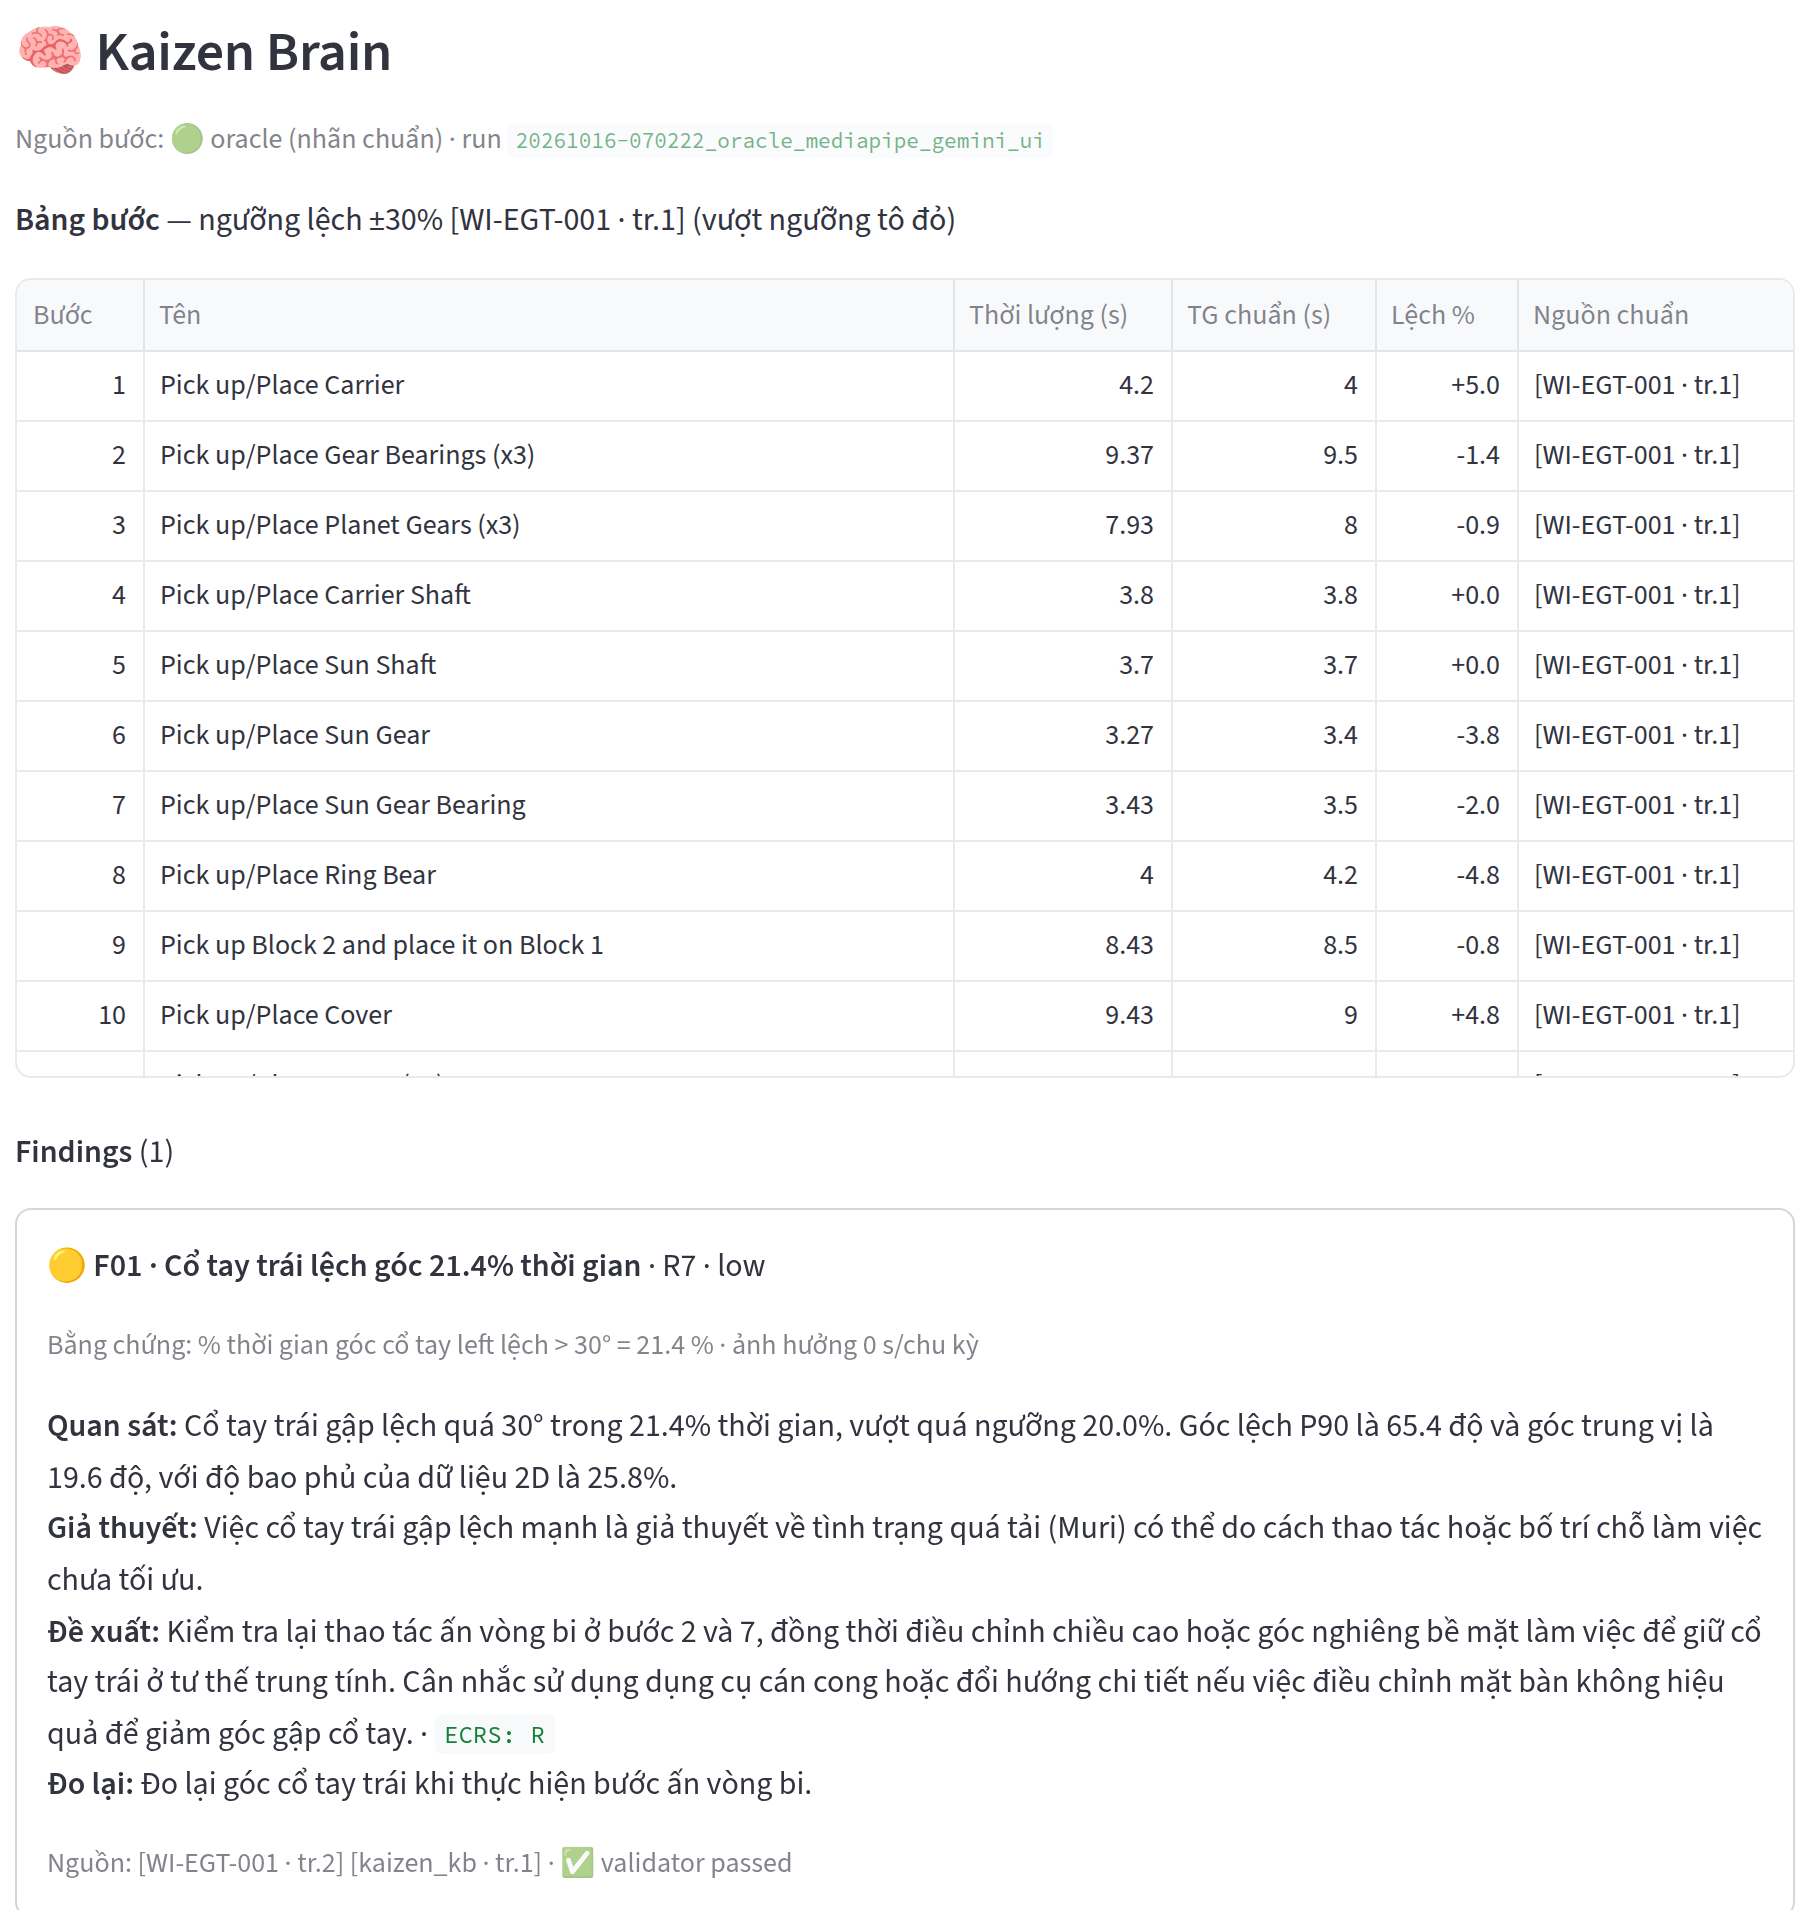
\includegraphics[width=0.75\textwidth]{ui2_brain.png}
  \caption{Trang ``Kaizen Brain'' của UI: bảng bước với thời gian chuẩn và nguồn trích dẫn, cùng một phát hiện R7
  kèm giải thích LLM đã qua validator.}
  \label{fig:ui}
\end{figure}

\subsection{Model Architectures}
\label{subsec:arch}
\textbf{Pose.} \Cref{tab:pose_models} liệt kê các backend.
MediaPipe Pose Landmarker \cite{mp_pose} chạy ở chế độ video. Hand Landmarker \cite{mp_hand}
có thể chạy trên vùng vuông quanh từng cổ tay, và tay được ghép với cổ tay gần nhất.
RTMW \cite{rtmlib} chạy qua rtmlib/ONNX.
Backend \code{rtmpose-custom} nạp một RTMPose-m \cite{rtmpose} đã fine-tune và export sang ONNX
(biến môi trường \code{KAIZEN\_POSE\_ONNX}).
Mọi backend ghi ra cùng một schema \code{.npz}: \code{kpts (T,K,3), t, names, meta}.

\begin{table}[t]
\centering
\caption{Các backend ước lượng khung xương}
\label{tab:pose_models}
\footnotesize
\setlength{\tabcolsep}{3pt}
\begin{tabularx}{\columnwidth}{@{}lcXl@{}}
\toprule
Backend & Điểm & Ghi chú & Muri \\
\midrule
MediaPipe (mặc định) & 75 & 33 thân + $2\times21$ tay; CPU & có \\
RTMW-m & 133 & toàn thân COCO-WholeBody; ONNX & có \\
RTMPose-m fine-tune & 17 & COCO-17, nhãn giả Kinect; không có điểm tay & không \\
\bottomrule
\end{tabularx}
\end{table}

\textbf{Đặc trưng cho segmenter (kp\_v1).} Mỗi frame dùng $J=15$ khớp: mũi, hai vai, hai khuỷu, hai cổ tay, hai hông,
và ba điểm của mỗi bàn tay (gốc ngón giữa, đầu ngón trỏ, đầu ngón cái).
Mỗi khớp cho 7 giá trị, nên vector đặc trưng có $D=7J=105$ chiều:
\begin{itemize}
  \item toạ độ tuyệt đối $(x/W,y/H)$, vì vị trí khay cố định theo camera;
  \item toạ độ theo thân $(p-\bar p_{\text{vai}})/\lVert p_{\text{vai,L}}-p_{\text{vai,R}}\rVert$;
  \item vận tốc $\Delta(x/W,y/H)\cdot f$;
  \item mask hợp lệ (score $\ge0{,}3$).
\end{itemize}
Khớp mà model pose không có (ví dụ COCO-17 không có bàn tay) nhận giá trị 0 và mask 0, nên $D$ luôn cố định.
Đặc trưng được chuẩn hoá z-score bằng thống kê của tập train, lưu cùng model.

\textbf{MS-TCN.} \Cref{fig:mstcn} mô tả kiến trúc, theo đúng thiết kế gốc \cite{farha2019mstcn}:
$S=4$ stage, mỗi stage $L=10$ lớp residual tích chập giãn (kernel 3, dilation $2^\ell$), 64 kênh, dropout 0{,}5.
Trường tiếp nhận của mỗi stage khoảng $2^{L+1}-1=2047$ frame (ở 15\,fps tương đương khoảng 136\,s), dài hơn một chu kỳ lắp.
Stage 2..$S$ nhận softmax của stage trước. Hàm mất mát của mỗi stage là
\begin{equation}
  \mathcal{L}_s=\frac{1}{T}\sum_t -\log \hat y_{t,c_t}
  + \frac{\lambda}{TC}\sum_{t,c}\min\!\big(\Delta_{t,c}^2,\tau^2\big),
  \label{eq:mstcn_loss}
\end{equation}
với $\Delta_{t,c}=\log\hat y_{t,c}-\log\hat y_{t-1,c}$, $\lambda=0{,}15$ và $\tau=4$.
Frame không có nhãn được bỏ qua khi tính loss.
Model có khoảng \todo{số tham số, in bằng \code{sum(p.numel())}} tham số.

\begin{figure}[t]
  \centering
  \resizebox{0.8\textwidth}{!}{% Kiến trúc MS-TCN dùng cho phân đoạn bước (TikZ) — dùng trong sections/04_implementation.tex
\begin{tikzpicture}[
  font=\scriptsize,
  >={Stealth[length=1.6mm]},
  blk/.style={draw, rounded corners=1.5pt, align=center, minimum height=0.6cm, inner sep=2pt},
  conv/.style={blk, fill=blue!8, minimum width=1.0cm},
  dil/.style={blk, fill=violet!10, minimum width=0.55cm},
  st/.style={draw=gray!70, dashed, rounded corners=3pt, inner sep=4pt},
]
% đầu vào
\node[blk, fill=gray!10, align=center] (x) at (0,0) {$X\!\in\!\mathbb{R}^{105\times T}$\\kp\_v1};
% stage 1
\node[conv, right=0.35cm of x] (in1) {1$\times$1\\conv};
\node[dil, right=0.25cm of in1] (d1) {$d{=}1$};
\node[dil, right=0.1cm of d1] (d2) {$d{=}2$};
\node[right=0.05cm of d2] (dots) {$\cdots$};
\node[dil, right=0.05cm of dots] (dL) {$2^{L-1}$};
\node[conv, right=0.25cm of dL] (out1) {1$\times$1\\conv};
\node[st, fit=(in1)(out1), label={[font=\scriptsize]above:Stage 1 (dự đoán ban đầu)}] (S1) {};
\draw[->] (x) -- (in1); \draw[->] (in1) -- (d1); \draw[->] (d1) -- (d2); \draw[->] (dL) -- (out1);

% stage 2..S
\node[blk, fill=orange!10, below=0.75cm of out1, minimum width=1.4cm] (sm) {softmax};
\node[blk, fill=violet!5, left=0.35cm of sm, minimum width=3.4cm] (S2) {Stage 2 \dots{} Stage $S$ (tinh chỉnh)\\cùng cấu trúc, vào $= C$ kênh};
\node[blk, fill=green!8, left=0.35cm of S2] (y) {$\hat{Y}_S\!\in\!\mathbb{R}^{C\times T}$};
\draw[->] (out1) -- node[right]{\tiny $\hat{Y}_1$} (sm);
\draw[->] (sm) -- (S2); \draw[->] (S2) -- (y);

% chi tiết lớp giãn
\node[draw, rounded corners=2pt, fill=violet!3, align=flush left, below=0.35cm of y.south west, anchor=north west,
      text width=6.3cm] (res) {
  \textbf{Lớp residual giãn} ($d=2^{\ell}$, $\ell=0..L-1$):\\
  \quad$h \leftarrow h + \mathrm{Dropout}\big(\mathrm{Conv}_{1\times1}(\mathrm{ReLU}(\mathrm{Conv}^{d}_{3}(h)))\big)$\\
  \textbf{Loss mỗi stage:} $\mathcal{L}_s = \mathcal{L}_{CE} + \lambda\,\mathcal{L}_{T\text{-}MSE}$ (cắt ở $\tau=4$);
  tổng $\sum_{s=1}^{S}\mathcal{L}_s$.};
\end{tikzpicture}
}
  \caption{MS-TCN cho phân đoạn bước. Đầu vào là chuỗi đặc trưng kp\_v1;
  $C$ lớp tương ứng các cặp (action, repetition) cộng lớp nền.}
  \label{fig:mstcn}
\end{figure}

\textbf{LLM và embedding.} Lớp provider thống nhất hỗ trợ Gemini (mặc định \code{gemini-2.5-flash}) \cite{gemini},
Anthropic Claude (\code{claude-sonnet-4-6}), OpenAI (\code{gpt-4.1-mini}, chế độ JSON)
và provider \code{dry-run}
để chạy không cần key.
Embedding dùng model \path{intfloat/multilingual-e5-small} \cite{e5}, chạy cục bộ.
Một embedder băm $n$-gram tất định được dùng cho CI và môi trường offline.

\subsection{Datasets}
\label{subsec:data}
\textbf{HA4M} \cite{ha4m} gồm 41 người lắp (U001--U041) bộ bánh răng hành tinh theo 12 hành động
(\cref{tab:actions}), được quay bằng Azure Kinect.
Bước 00 của pipeline đọc trực tiếp dữ liệu thật để chốt schema, thay vì giả định. Kết quả:
{\raggedright
\begin{itemize}
  \item mỗi lần lắp nằm trong thư mục \code{IDU<subject>V<trial>/};
  \item ảnh Color là chuỗi PNG $2048\times1536$, tên dạng \code{FrameID<6 số>\_DeviceTimeStamp<µs>us.png};
        fps\,=\,30, xác nhận bằng trung vị $\Delta t$\,=\,33{,}33\,ms;
  \item \code{Labels.txt} có ba cột nguyên phân tách bằng dấu cách: \code{frame action\_id repetition},
        với 0 là ``don't care'';
  \item skeleton Kinect lưu dạng TSV 32 khớp, có toạ độ chiếu lên ảnh Color.
\end{itemize}
\par}
Mỗi thư mục lần lắp chiếm khoảng 18\,GB vì có đủ mọi modality, nhưng pipeline chỉ cần Color và nhãn
(thêm Skeletons cho phần fine-tune pose).
Sau khi trích keypoint, phần huấn luyện chỉ cần file \code{.npz} (khoảng 1{,}3\,MB mỗi video) và \code{Labels.txt}.

\begin{table}[t]
\centering
\caption{12 hành động HA4M và số frame của U001\_V001}
\label{tab:actions}
\footnotesize
\setlength{\tabcolsep}{3pt}
\begin{tabularx}{\columnwidth}{@{}clcr@{}}
\toprule
ID & Hành động & Lặp & Frame \\
\midrule
1 & Pick up/Place Carrier & 1 & 126 \\
2 & Pick up/Place Gear Bearings & 3 & 281 \\
3 & Pick up/Place Planet Gears & 3 & 238 \\
4 & Pick up/Place Carrier Shaft & 1 & 114 \\
5 & Pick up/Place Sun Shaft & 1 & 111 \\
6 & Pick up/Place Sun Gear & 1 & 98 \\
7 & Pick up/Place Sun Gear Bearing & 1 & 103 \\
8 & Pick up/Place Ring Bear & 1 & 120 \\
9 & Pick up Block 2, place on Block 1 & 1 & 253 \\
10 & Pick up/Place Cover & 1 & 283 \\
11 & Pick up/Place Screw & 2 & 291 \\
12 & Allen key: turn screws, return key \& EGT & 1 & 319 \\
\midrule
0 & Don't care (đầu/cuối) & -- & 90 \\
\bottomrule
\end{tabularx}
\end{table}

\textbf{Dữ liệu đã dùng.} Hiện tại có hai lần lắp của U001: V001 (2427 frame, 80{,}9\,s) và V002 (2655 frame).
Dữ liệu cho phần huấn luyện: \todo{danh sách subject/trial đã tải, ví dụ U001--U005, tổng số video, tổng số frame}.

\textbf{Cấu hình trạm.} File \code{station.yaml} khai báo 11 zone (10 khay và vùng lắp).
Mỗi zone là vùng \textit{cổ tay} khi với vào khay, không phải viền khay, và được vẽ bằng công cụ click chuột trên một frame
(\cref{fig:station}).
File còn khai báo 12 bước SOP ứng với khay đặc trưng (bước 9 không có khay), cờ VA, ROI chạy pose
và các ngưỡng ở \cref{sec:method}.

\textbf{Tri thức.} Kho tri thức gồm ba nguồn:
\code{kaizen\_kb.md} có 16 đoạn \code{[KB-xx]} (3M, 7 lãng phí, nguyên tắc Barnes, ECRS, Standardized Work, Yamazumi);
\code{sop.md} có 16 đoạn \code{[SOP-xx]} mô phỏng SOP 12 bước;
và work instruction mô phỏng \code{WI-EGT-001} (PDF 2 trang) có bảng thời gian chuẩn từng bước, ngưỡng lệch 30\%
và ngưỡng góc cổ tay 30°.

\begin{figure}[t]
  \centering
  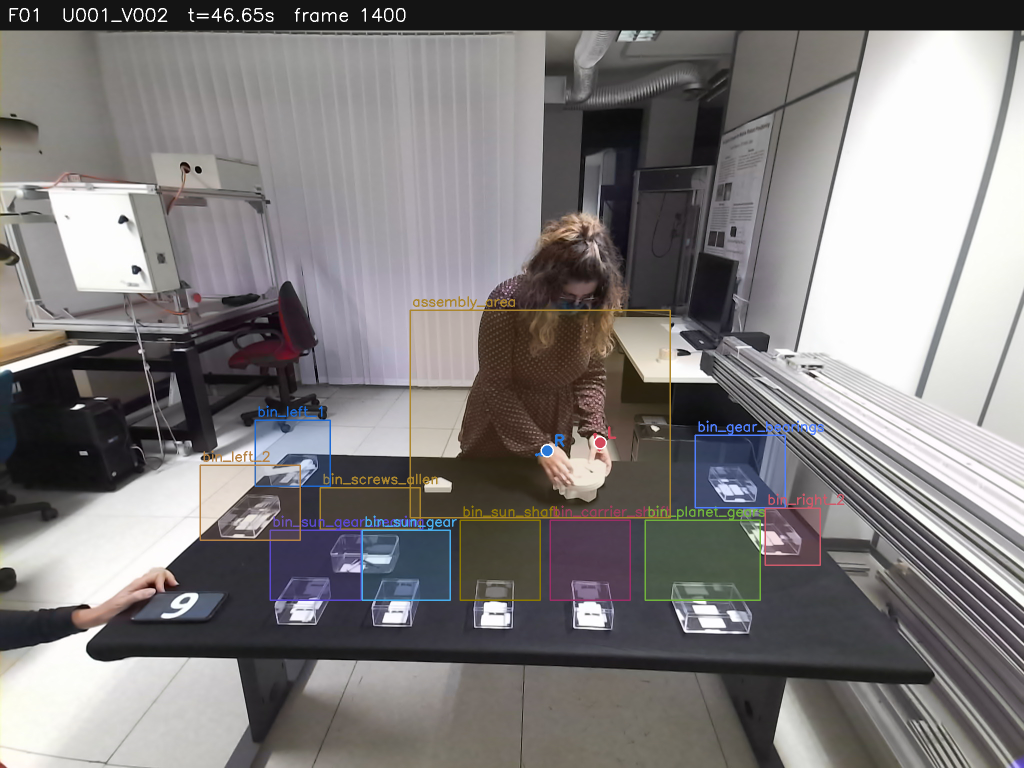
\includegraphics[width=0.85\textwidth]{evidence_F01.png}
  \caption{Trạm HA4M (U001\_V002, frame 1400) với 11 zone đã cấu hình và hai cổ tay (L/R) ước lượng bằng MediaPipe.
  Ảnh này là ảnh bằng chứng do khối 08 tự sinh cho một phát hiện.}
  \label{fig:station}
\end{figure}

\subsection{Training}
\label{subsec:training}
% ---------------------------------------------------------------
% DRAFT — điền số liệu sau khi tự chạy các lệnh trong docs/training.md
% ---------------------------------------------------------------
Huấn luyện là \textit{tuỳ chọn} và chỉ chạy khi người dùng gõ lệnh.
Khi chưa có model, pipeline vẫn dùng đường mặc định (pose pretrained, tách bước bằng quy tắc).

\textbf{Segmenter MS-TCN.} Tập dữ liệu được quét từ các cặp \code{.npz} và \code{Labels.txt}.
Nhãn được căn theo chỉ số frame của \code{.npz}.
Dữ liệu được chia train/val/test \textit{theo người lắp}, nên không người nào xuất hiện ở hai tập.
Đánh giá chéo dùng group $k$-fold theo người, hoặc leave-one-subject-out (LOSO, $k=0$).
Siêu tham số mặc định theo MS-TCN gốc (\cref{tab:hparams}).
Model được huấn luyện ở 15\,fps (lấy 1 trong 2 frame); khi dự đoán, nhãn được lặp lại về 30\,fps.
Huấn luyện dừng sớm theo F1@50 trên tập val.
Thư mục model lưu \code{model.pt}, \code{config.json} và \code{train\_log.csv}.
\code{config.json} gồm danh sách lớp, thống kê chuẩn hoá, danh sách người của từng tập, siêu tham số, epoch tốt nhất
và đánh giá mức bước trên val, theo cùng định nghĩa với khối 04.
\begin{Verbatim}[fontsize=\scriptsize,frame=single]
python -m kaizen.train.segmenter status
python -m kaizen.train.segmenter cv --folds 0
python -m kaizen.train.segmenter train --name mstcn_v1 \
       --val-subjects <S_val> --test-subjects <S_test>
\end{Verbatim}

\begin{table}[t]
\centering
\caption{Siêu tham số huấn luyện MS-TCN}
\label{tab:hparams}
\footnotesize
\begin{tabular}{@{}ll@{}}
\toprule
Tham số & Giá trị \\
\midrule
Stage / lớp / kênh & 4 / 10 / 64 \\
Dropout & 0{,}5 \\
$\lambda$ (làm mượt), $\tau$ & 0{,}15, 4 \\
Optimizer & Adam, lr $5\!\times\!10^{-4}$, weight decay $10^{-4}$ \\
Batch / epoch tối đa & 4 video / 100 \\
Early stopping & patience 20 epoch theo F1@50 (val) \\
Lấy mẫu & 1/2 (15\,fps) \\
Hậu xử lý & nhập mảnh bước $<0{,}5$\,s \\
Phần cứng & \todo{CPU/GPU, số lõi, RAM} \\
Thời gian train & \todo{phút/lần train; tổng cho CV} \\
\bottomrule
\end{tabular}
\end{table}

\todo{Đường cong loss và F1@50 (val) theo epoch, vẽ từ \code{train\_log.csv}, lưu \code{figures/train\_curve.png}
rồi bỏ comment khối figure bên dưới.}
% \begin{figure}[t]
%   \centering
%   \includegraphics[width=\columnwidth]{train_curve.png}
%   \caption{Loss train và F1@50 trên val theo epoch (MS-TCN).}
%   \label{fig:train_curve}
% \end{figure}

\textbf{Fine-tune RTMPose (nhãn giả Kinect).} Skeleton Azure Kinect đã chiếu lên ảnh Color được ánh xạ sang 17 khớp COCO.
Khớp có độ tin cậy $\ge0{,}5$ nhận visibility 2; khớp có độ tin cậy dương nhưng thấp hơn nhận visibility 1.
Cứ 15 frame lấy 1 frame; frame có ít nhất 6 khớp nhìn thấy được giữ lại.
Ảnh được crop quanh người (lề 25\%) và lưu thành JPEG kèm annotation COCO.
Model khởi tạo từ RTMPose-m pretrained trên COCO và AIC, được fine-tune 60 epoch với lr $10^{-4}$ và EMA trong MMPose
\cite{rtmpose}, rồi export ONNX bằng MMDeploy.
Nhãn giả mang theo sai số của Kinect, nhất là ở cổ tay khi bị che.
Vì vậy model fine-tune chỉ được giữ lại nếu PCK so với Kinect trên người lắp chưa thấy tốt hơn baseline.
Số liệu: \todo{số ảnh train/val, số người, thời gian train, GPU}.

% ============================== V. EXPERIMENTS AND RESULTS ==============================
% Số liệu đã đo lấy từ run 20261016-055308_oracle_mediapipe_gemini_rag-report-2t (oracle + eval pred),
% outputs/kinect_compare_U001_V001.json và `python -m kaizen.train.pose eval` (MediaPipe, U001_V002).
% Ô \tbd = DRAFT, điền sau khi train/đánh giá trên nhiều subject.
\section{Experiments and Results}
\label{sec:exp}

\subsection{Thiết lập thực nghiệm}
\label{subsec:setup}
\textbf{Dữ liệu.} Kết quả ở mục này được đo trên U001\_V001 và U001\_V002 của HA4M.
Thực nghiệm huấn luyện dùng \todo{tập subject, cách chia train/val/test hoặc LOSO}.
\textbf{Phần cứng.} \todo{CPU (số lõi), RAM, GPU nếu có}. Mọi bước suy luận trong bài chạy trên CPU.
\textbf{Chỉ số.}
\begin{itemize}
  \item Pose: sai số pixel so với skeleton Kinect (trung vị, P90, tỷ lệ frame lệch $<50$\,px) và PCK@$\alpha$.
        PCK@$\alpha$ là tỷ lệ khớp có sai số $<\alpha$ lần cạnh dài của khung người.
  \item Phân đoạn bước: \Fone, MAE thời lượng bước, MAE mốc bắt đầu và kết thúc, sai số cycle time.
        Với MS-TCN báo thêm độ chính xác frame, Edit và F1@\{10,25,50\} \cite{farha2019mstcn}.
  \item LLM: tỷ lệ đạt validator ngay lần đầu và sau khi hỏi lại.
\end{itemize}

\subsection{Độ chính xác ước lượng cổ tay}
\label{subsec:exp_pose}
Bảng~\ref{tab:kinect} so sánh cổ tay MediaPipe với skeleton Kinect đã chiếu lên ảnh Color.
Lưu ý rằng skeleton Kinect cũng là một ước lượng.
Tay phải bám tốt: trung vị 24{,}5\,px và 95{,}1\% frame lệch dưới 50\,px, tức nhỏ hơn kích thước một khay trên ảnh $2048\times1536$.
Tay trái kém tin cậy hơn (P90 151{,}6\,px) vì thường bị thân người và cụm lắp che.
Tỷ lệ phát hiện người đạt 0{,}953 (V001) và 0{,}961 (V002).
Trên U001\_V002, MediaPipe đạt PCK@0{,}05 bằng 58{,}4 và PCK@0{,}1 bằng 77{,}6 (trung bình mọi khớp COCO-17).
Sai số trung vị là 23{,}3\,px ở cổ tay phải và 26{,}6\,px ở cổ tay trái.

\begin{table}[t]
\centering
\caption{Cổ tay MediaPipe so với skeleton Azure Kinect (U001\_V001)}
\label{tab:kinect}
\footnotesize
\begin{adjustbox}{max width=\columnwidth}
\begin{tabular}{@{}lrrrr@{}}
\toprule
Tay & Số frame & Trung vị (px) & P90 (px) & $<$50\,px (\%) \\
\midrule
Trái & 2148 & 26{,}1 & 151{,}6 & 77{,}7 \\
Phải & 2314 & 24{,}5 & 43{,}4 & 95{,}1 \\
\bottomrule
\end{tabular}
\end{adjustbox}
\end{table}

\begin{table}[t]
\centering
\caption{PCK so với Kinect trên người lắp chưa thấy (DRAFT)}
\label{tab:pck}
\footnotesize
\setlength{\tabcolsep}{3pt}
\begin{adjustbox}{max width=\columnwidth}
\begin{tabular}{@{}lcccc@{}}
\toprule
Backend & PCK@0{,}05 & PCK@0{,}1 & L-wrist (px) & R-wrist (px) \\
\midrule
MediaPipe (U001\_V002) & 58{,}4 & 77{,}6 & 26{,}6 & 23{,}3 \\
RTMW-m & \tbd & \tbd & \tbd & \tbd \\
RTMPose-m fine-tune & \tbd & \tbd & \tbd & \tbd \\
\bottomrule
\end{tabular}
\end{adjustbox}
\end{table}

\subsection{Phân đoạn bước}
\label{subsec:exp_seg}
\textbf{Baseline quy tắc.} \Cref{tab:seg} cho kết quả của baseline quy tắc (\cref{alg:rule}) so với nhãn HA4M.
Trên V001, 15/17 đoạn được neo, với \Fone{} 0{,}75, MAE thời lượng 0{,}62\,s và sai số cycle time 0{,}6\,s.
Trên V002, lần lặp thứ ba của bước 3 (3.2) và bước 5 không được neo, nên chỉ có 11/17 đoạn; \Fone{} đạt 0{,}714 và sai số cycle time 2{,}27\,s.
Phân tích lỗi cho thấy ba nguồn chính:
\begin{enumerate}
  \item bước 9 không có khay đặc trưng nên không có mốc;
  \item mốc bắt đầu bước 10 trễ 4{,}77\,s (V001) và 3{,}13\,s (V002), vì công nhân với tới khay nắp trước khi
        kết thúc thao tác bước 9;
  \item mốc kết thúc bước 12 lệch 2--3{,}5\,s, do bước 12 gồm cả việc trả lục giác và sản phẩm, không có sự kiện neo rõ.
\end{enumerate}
Các bước 1--8 có IoU từ 0{,}43 tới 0{,}80 và độ lệch mốc thường dưới 1\,s.

\begin{table}[t]
\centering
\caption{Phân đoạn bước so với nhãn HA4M. Dòng MS-TCN là DRAFT.}
\label{tab:seg}
\footnotesize
\setlength{\tabcolsep}{2.5pt}
\begin{adjustbox}{max width=\columnwidth}
\begin{tabular}{@{}llcccccc@{}}
\toprule
Phương pháp & Trial & Bước & \Fone & MAE dur & MAE start & MAE end & $\lvert\Delta$CT$\rvert$ \\
            &       & neo/nhãn & & (s) & (s) & (s) & (s) \\
\midrule
Rule & V001 & 15/17 & 0{,}750 & 0{,}62 & 1{,}11 & 0{,}87 & 0{,}60 \\
Rule & V002 & 11/17 & 0{,}714 & 0{,}92 & 0{,}80 & 1{,}05 & 2{,}27 \\
\midrule
MS-TCN (LOSO) & \tbd & \tbd & \tbd & \tbd & \tbd & \tbd & \tbd \\
MS-TCN (test) & \tbd & \tbd & \tbd & \tbd & \tbd & \tbd & \tbd \\
\bottomrule
\end{tabular}
\end{adjustbox}
\end{table}

\textbf{MS-TCN (DRAFT).}
\Cref{tab:mstcn} được điền từ đầu ra của \code{segmenter cv} và \code{segmenter eval}.
\todo{Nhận xét: MS-TCN có tách được bước 9 (không khay) và sửa mốc bước 10, 12 hay không;
so sánh \Fone{} với baseline 0{,}75/0{,}714; phân mảnh đoạn (Edit) trước và sau khi làm mượt.}

\begin{table}[t]
\centering
\caption{MS-TCN, chỉ số chuẩn phân đoạn hành động (DRAFT)}
\label{tab:mstcn}
\footnotesize
\setlength{\tabcolsep}{3pt}
\begin{adjustbox}{max width=\columnwidth}
\begin{tabular}{@{}lccccc@{}}
\toprule
Thiết lập & Acc & Edit & F1@10 & F1@25 & F1@50 \\
\midrule
LOSO, \tbd{} người & \tbd & \tbd & \tbd & \tbd & \tbd \\
Test giữ riêng & \tbd & \tbd & \tbd & \tbd & \tbd \\
Ablation: không $\mathcal{L}_{T\text{-}MSE}$ & \tbd & \tbd & \tbd & \tbd & \tbd \\
Ablation: $S=1$ stage & \tbd & \tbd & \tbd & \tbd & \tbd \\
Ablation: chỉ toạ độ theo thân & \tbd & \tbd & \tbd & \tbd & \tbd \\
\bottomrule
\end{tabular}
\end{adjustbox}
\end{table}

\begin{figure}[t]
  \centering
  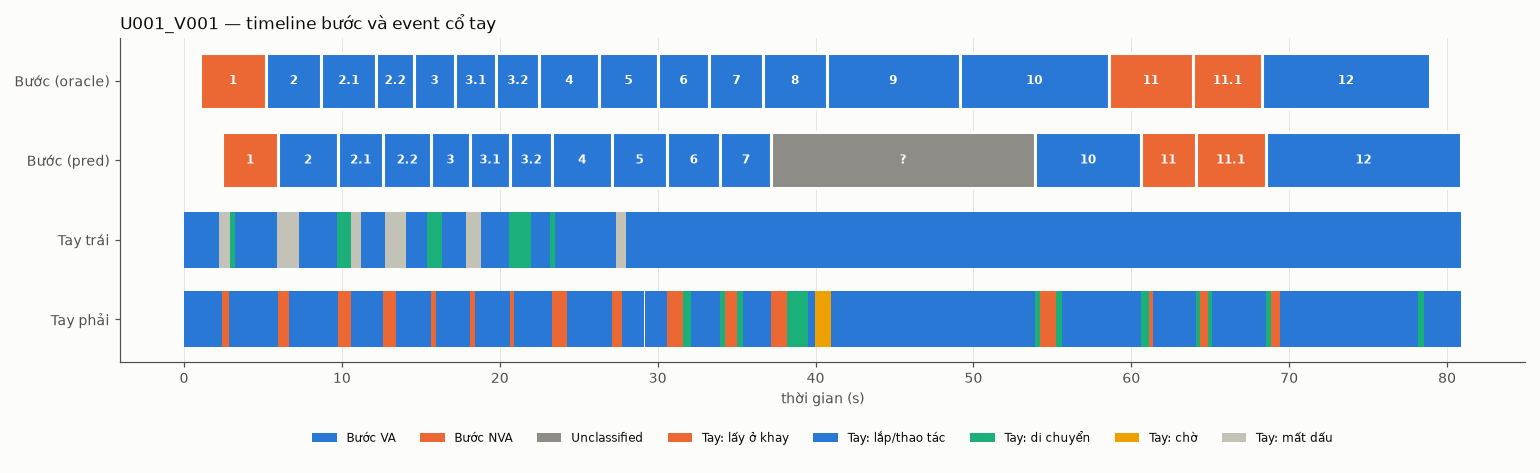
\includegraphics[width=0.9\textwidth]{gantt_U001_V001.png}\\[4pt]
  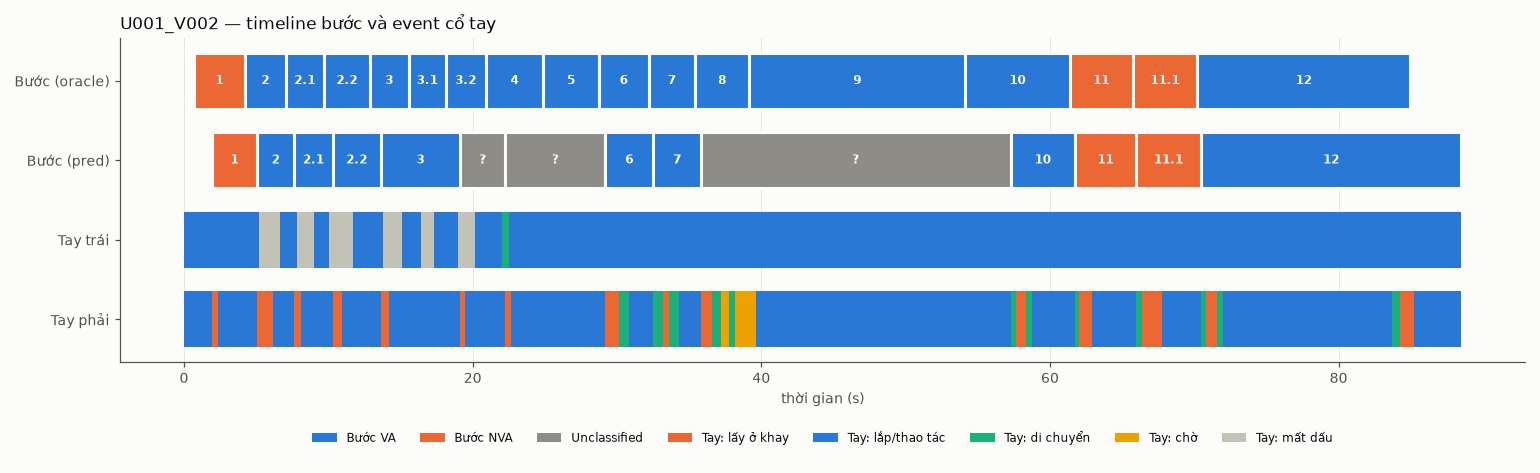
\includegraphics[width=0.9\textwidth]{gantt_U001_V002.png}
  \caption{Timeline Gantt các bước: nhãn HA4M (oracle) so với dự đoán bằng quy tắc, U001\_V001 (trên) và U001\_V002 (dưới).}
  \label{fig:gantt}
\end{figure}

\subsection{Chỉ số Kaizen và phát hiện: nghiên cứu tình huống}
\label{subsec:exp_case}
Ở chế độ oracle, cycle time là 77{,}9\,s (V001) và 84{,}3\,s (V002).
Trung bình là 81{,}1\,s với CV 0{,}056, dưới ngưỡng R6 (0{,}25).
\%VA đạt 82{,}1\% và 85{,}3\%.
Số lần lấy là 15 và 14.
Quãng đường cổ tay trái và phải là 18\,660 và 13\,715\,px (V001).
\Cref{fig:yamazumi} cho thấy thời lượng bước khá ổn định giữa hai lần lắp, trừ bước 9 (CV 0{,}395) và bước 12 (CV 0{,}231).

So với thời gian chuẩn trong work instruction, V001 nằm trong ngưỡng $\pm30\%$ ở mọi bước (lệch từ $-4{,}8\%$ tới $+5{,}0\%$).
V002 kích hoạt hai phát hiện R8:
\begin{itemize}
  \item bước 9 mất 14{,}97\,s so với chuẩn 8{,}5\,s ($+76{,}1\%$; ảnh hưởng 6{,}47\,s/chu kỳ);
  \item bước 12 mất 14{,}77\,s so với chuẩn 11\,s ($+34{,}3\%$; 3{,}77\,s/chu kỳ).
\end{itemize}
R2 phát hiện thêm một lần lấy dư ở khay vít/lục giác (0{,}78\,s/chu kỳ).
Tổng tiềm năng cải thiện là 5{,}5\,s/chu kỳ, tính bằng cộng thô ảnh hưởng của các phát hiện, chưa khử trùng lặp.
Về Muri (\cref{tab:muri}), tay phải được đo trên gần 90\% frame và lệch $>30^\circ$ trong 11{,}5--15{,}2\% thời gian.
Tay trái chỉ đo được khoảng 25\% frame vì điểm bàn tay hay mất. Vì vậy R7 chỉ đánh giá độ tin cậy \textit{low}
và báo kèm độ phủ.
R1 bị bỏ qua vì cần ít nhất 3 trial; R4 ở chế độ oracle xác nhận chuỗi nhãn khớp SOP 12 bước.

\begin{figure}[t]
  \centering
  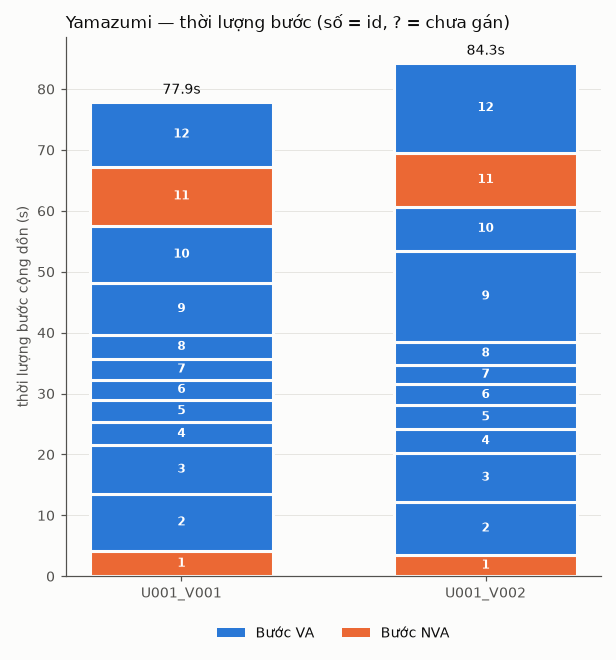
\includegraphics[width=0.8\textwidth]{yamazumi.png}
  \caption{Biểu đồ Yamazumi: thời lượng các bước chồng theo trial (oracle).}
  \label{fig:yamazumi}
\end{figure}

\begin{table}[t]
\centering
\caption{Muri: góc cổ tay 2D (sàng lọc)}
\label{tab:muri}
\footnotesize
\setlength{\tabcolsep}{3pt}
\begin{adjustbox}{max width=\columnwidth}
\begin{tabular}{@{}llrrrr@{}}
\toprule
Trial & Tay & Phủ (\%) & Trung vị (°) & $>30^\circ$ (\%) & P90 $\Delta$ (°) \\
\midrule
V001 & trái & 25{,}8 & 19{,}6 & 21{,}4 & 65{,}4 \\
V001 & phải & 86{,}9 & 17{,}5 & 11{,}5 & 32{,}8 \\
V002 & trái & 25{,}0 & 15{,}8 & 17{,}1 & 70{,}7 \\
V002 & phải & 89{,}9 & 18{,}5 & 15{,}2 & 38{,}1 \\
\bottomrule
\end{tabular}
\end{adjustbox}
\end{table}

\begin{figure}[t]
  \centering
  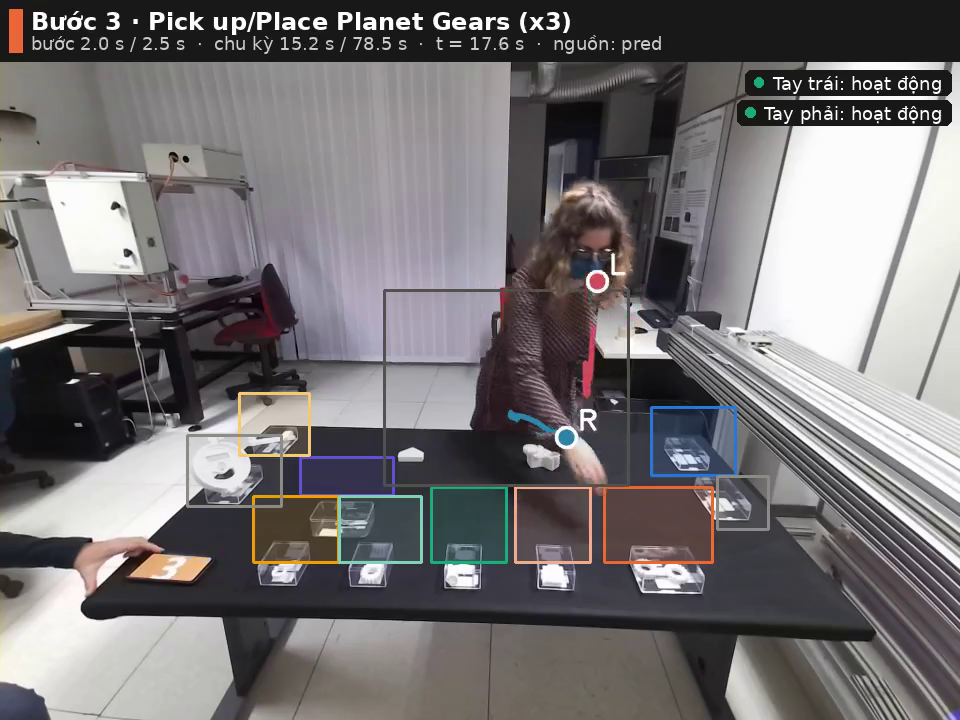
\includegraphics[width=0.8\textwidth]{frame_V001_step3.png}
  \caption{Video overlay sinh tự động: bước hiện tại, tiến độ trong bước và chu kỳ, trạng thái hai tay, zone và vệt cổ tay
  (U001\_V001, bước 3).}
  \label{fig:overlay}
\end{figure}

\subsection{Diễn giải LLM có kiểm chứng}
\label{subsec:exp_llm}
\Cref{tab:llm} tổng hợp tỷ lệ đạt validator qua các run.
Trong run có 4 phát hiện với RAG, Gemini 2.5 Flash đạt 3/4 ngay lần đầu.
Câu trả lời còn lại đạt sau một lần hỏi lại có phản hồi lỗi, nên tỷ lệ cuối là 100\%.
Mọi trích dẫn đều là \code{chunk\_id} có trong kho, và bảng tài liệu tham chiếu khớp hai chiều với các nhãn trong báo cáo.
Một bài học thực tế: ở lần chạy Gemini đầu tiên, câu ``phân vị 90'' bị đánh trượt oan
vì số 90 chỉ xuất hiện trong tên trường \code{dev\_p90\_deg}.
Sau khi bổ sung tập $\mathcal{N}(f)$ vào whitelist (\cref{eq:whitelist}), lỗi này không còn.
Validator không bắt được lỗi \textit{ngữ nghĩa}, ví dụ một con số có thật nhưng được gán sai ý.
Phần này vẫn cần kỹ sư IE duyệt.

\begin{table}[t]
\centering
\caption{Tỷ lệ đạt validator của tầng LLM}
\label{tab:llm}
\footnotesize
\setlength{\tabcolsep}{3pt}
\begin{adjustbox}{max width=\columnwidth}
\begin{tabular}{@{}llccc@{}}
\toprule
Provider / model & Ngữ cảnh & \#finding & Lần đầu & Sau retry \\
\midrule
Gemini 2.5 Flash & RAG (WI + KB) & 4 & 75\% & 100\% \\
Gemini 2.5 Flash & RAG & 1 & 100\% & 100\% \\
Gemini 3.8 Flash & KB/SOP tĩnh & 1 & 100\% & 100\% \\
Claude Sonnet 4.6 & RAG & \tbd & \tbd & \tbd \\
GPT-4.1 mini & RAG & \tbd & \tbd & \tbd \\
\bottomrule
\end{tabular}
\end{adjustbox}
\end{table}

\subsection{Thời gian chạy}
\label{subsec:exp_runtime}
Trên CPU, việc trích keypoint MediaPipe đạt khoảng 7{,}2--7{,}6\,fps, tức khoảng 6 phút cho mỗi video 80\,s.
Đây là bước chậm nhất, và kết quả được tái sử dụng giữa các run.
Các bước 02$\to$08 mất khoảng 8--9\,s cho 2 trial, chưa tính thời gian gọi LLM.
Render video overlay mất khoảng 2 phút mỗi video.
Suy luận MS-TCN: \todo{ms/video trên CPU}.
So với 2--4 giờ bấm giờ thủ công cho mỗi trạm, hệ thống cho số liệu của mọi chu kỳ đã quay,
thay vì chỉ vài chu kỳ được lấy mẫu.

\subsection{Thảo luận và giới hạn}
\label{subsec:limits}
\begin{itemize}
  \item \textbf{Quy mô dữ liệu.} Các số liệu đo được mới chỉ từ hai lần lắp của một người.
        Các chỉ số Mura giữa người và R1 cần nhiều trial và nhiều người hơn mới có ý nghĩa thống kê.
  \item \textbf{Phụ thuộc cấu hình trạm.} Zone được vẽ tay cho một camera cố định.
        Baseline quy tắc không tách được bước không có khay.
        Đặc trưng kp\_v1 dùng cả toạ độ tuyệt đối, nên một trạm hoặc camera mới cần dữ liệu có nhãn để train lại.
  \item \textbf{Đơn vị và hiệu chuẩn.} Quãng đường đang tính theo pixel (\code{px\_per\_cm}\,=\,null).
        Ngưỡng moving/still (120\,px/s) được chỉnh theo đồ thị tốc độ, chưa hiệu chuẩn hệ thống.
  \item \textbf{Muri 2D.} Góc chiếu phụ thuộc hướng camera, và tay trái chỉ đo được khoảng 25\% số frame.
        Chỉ số này chỉ dùng để sàng lọc.
  \item \textbf{Nhãn giả cho pose.} Fine-tune bằng skeleton Kinect có thể học cả sai số của Kinect.
\end{itemize}

% Sinh từ cùng nguồn nội dung với bản Word.
\section{Conclusion}

Nhóm đã xây dựng một hệ thống chạy trọn từ video lắp ráp đến báo cáo khuyến nghị có trích dẫn: trích điểm khớp, phân đoạn bước bằng MS-TCN, đo thời gian và ba chỉ số 3M, truy xuất tài liệu chuẩn và sinh diễn giải có kiểm tra. Hướng kết hợp phân đoạn hành động với RAG có giá trị cho Kaizen: mỗi con số trong báo cáo truy được về đoạn video và đoạn tài liệu đã tạo ra nó.

Trên người chưa thấy khi huấn luyện, MS-TCN vượt luật vùng khay (F1@50 34,3 so với 0, Acc 44,5\% so với 2,5\%), dù luật này là đối chứng yếu vì vùng khay được vẽ theo U001. Các nguyên nhân suy giảm mà nhóm xác định được đều nằm ở dữ liệu đầu vào: găng tay xoá phần lớn điểm ngón tay và người kiểm tra làm chậm hơn khoảng 1,5 lần. Bỏ điểm ngón tay và co giãn tốc độ nâng F1@50 từ 17,6 lên 34,3, giảm MAE thời lượng bước từ 4,23 xuống 2,80 giây. Ở tầng RAG, việc tách vai trò hoạt động đúng thiết kế: chương trình tính số, mô hình ngôn ngữ diễn giải, bộ kiểm tra chặn một con số không có trong dữ liệu phát hiện.

Phần chưa đạt nằm ở khả năng khái quát và độ tin cậy của đầu ra. F1@50 giảm từ 79,1 khi kiểm định chéo trong U001 xuống 34,3 trên U002, và kiểm định chéo trong một người không chọn ra cấu hình chỉ thân, cấu hình đạt 54,5 trên U002. Sai số phân đoạn đi qua được bộ kiểm tra: 3 trong 7 phát hiện lệch chuẩn không đúng so với ranh giới chuẩn, trong đó hai bước bị báo nhanh hơn chuẩn trong khi thực tế chậm hơn, và \%VA của U002 bị đo thành 92,1\% thay vì 73,9\%.

Ba hạn chế chính, trong đó lớn nhất là dữ liệu:
\begin{enumerate}\setlength{\itemsep}{1pt}
\item \textbf{Dữ liệu ít người.} Bộ dữ liệu quá nặng so với điều kiện của nhóm: mỗi video HA4M nén khoảng 12 GB, cả bộ 217 video khoảng 2,6 TB, trong khi ổ lưu trữ dùng chung chỉ còn 16–32 GB trống; nhóm phải xử lý tuần tự từng video; trích điểm khớp cho cả bộ sẽ mất khoảng 23 giờ CPU. Đến nay mới có 3 video của 2 người, khoảng 1,4\% bộ dữ liệu, trong đó một video bị hỏng phần cuối. Với một người huấn luyện và một người kiểm tra, nhóm chưa tách được ảnh hưởng của mô hình khỏi ảnh hưởng của người thao tác.
\item \textbf{Mô hình chưa khái quát tốt và chưa chạy thời gian thực.} Một video khoảng 2 phút cần khoảng 8–9 phút xử lý, và MS-TCN cần phần video phía sau thời điểm đang xét, nên hệ thống hiện chỉ phân tích video đã ghi.
\item \textbf{RAG và chỉ số Kaizen chưa được xác thực ngoài thực tế.} Kho tri thức là tài liệu mô phỏng 8 đoạn do nhóm biên soạn; bộ kiểm tra không xét đoạn được trích dẫn có hỗ trợ nhận định hay không; góc cổ tay 2D chỉ dùng để sàng lọc; và chưa có chuyên gia hay dữ liệu vận hành nào xác nhận các phát hiện.
\end{enumerate}

Nếu tiếp tục, nhóm ưu tiên thêm dữ liệu từ U003 trở đi và chọn mô hình bằng xác thực trên một người khác; sau đó xác nhận cấu hình chỉ thân kết hợp co giãn tốc độ; thử đặc trưng bền với găng tay (bộ phát hiện bàn tay tinh chỉnh trên ảnh có găng, hoặc chỉ dùng cổ tay với toạ độ tương đối theo vùng khay); xây tập truy vấn có nhãn để đánh giá truy xuất và việc trích dẫn có hỗ trợ nhận định; và hạ mức ưu tiên các phát hiện nằm ở vùng mô hình kém chắc chắn.


\clearpage
\addcontentsline{toc}{section}{References}
\bibliographystyle{IEEEtran}
{\raggedright\bibliography{references}\par}

\end{document}
